\documentclass[leqno, openany]{memoir}
\setulmarginsandblock{3.5cm}{3.5cm}{*}
\setlrmarginsandblock{3cm}{3.5cm}{*}
\checkandfixthelayout

\usepackage{amsmath}
\usepackage{amssymb}
\usepackage{amsthm}
%\usepackage{MnSymbol}
\usepackage{bm}
\usepackage{accents}
\usepackage{mathtools}
\usepackage{tikz}
\usetikzlibrary{calc}
\usetikzlibrary{automata,positioning}
\usepackage{tikz-cd}
\usepackage{forest}
\usepackage{braket} 
\usepackage{listings}
\usepackage{mdframed}
\usepackage{verbatim}
\usepackage{physics}
\usepackage{ytableau}
\usepackage{caption}
\usepackage{subcaption}
\usepackage{dynkin-diagrams}
\usepackage{rank-2-roots}

%font
\usepackage[sc]{mathpazo}
\usepackage{eulervm}
\usepackage[scaled=0.86]{berasans} 
\usepackage{inconsolata}
\usepackage{microtype}

%CS packages
\usepackage{algorithmicx}
\usepackage{algpseudocode}
\usepackage{algorithm}

% typeset and bib
\usepackage[english]{babel} 
\usepackage[utf8]{inputenc} 
\usepackage[T1]{fontenc} 
\usepackage[backend=biber, style=alphabetic]{biblatex}
\usepackage[bookmarks, colorlinks, breaklinks]{hyperref} 
\hypersetup{linkcolor=black,citecolor=black,filecolor=black,urlcolor=black}

% other formatting packages
\usepackage{float}
\usepackage{booktabs}
\usepackage{enumitem}
\usepackage{csquotes}
\usepackage{titlesec}
\usepackage{titling}
\usepackage{fancyhdr}
\usepackage{lastpage}
\usepackage{parskip}

\usepackage{lipsum}

% delimiters
\DeclarePairedDelimiter{\gen}{\langle}{\rangle}
\DeclarePairedDelimiter{\floor}{\lfloor}{\rfloor}
\DeclarePairedDelimiter{\ceil}{\lceil}{\rceil}


\newtheorem{thm}{Theorem}[section]
\newtheorem{cor}[thm]{Corollary}
\newtheorem{prop}[thm]{Proposition}
\newtheorem{lem}[thm]{Lemma}
\newtheorem{conj}[thm]{Conjecture}
\newtheorem{quest}[thm]{Question}

\theoremstyle{definition}
\newtheorem{defn}[thm]{Definition}
\newtheorem{defns}[thm]{Definitions}
\newtheorem{con}[thm]{Construction}
\newtheorem{exm}[thm]{Example}
\newtheorem{exms}[thm]{Examples}
\newtheorem{notn}[thm]{Notation}
\newtheorem{notns}[thm]{Notations}
\newtheorem{addm}[thm]{Addendum}
\newtheorem{exer}[thm]{Exercise}

\theoremstyle{remark}
\newtheorem{rmk}[thm]{Remark}
\newtheorem{rmks}[thm]{Remarks}
\newtheorem{warn}[thm]{Warning}
\newtheorem{sch}[thm]{Scholium}


% unnumbered theorems
\theoremstyle{plain}
\newtheorem*{thm*}{Theorem}
\newtheorem*{prop*}{Proposition}
\newtheorem*{lem*}{Lemma}
\newtheorem*{cor*}{Corollary}
\newtheorem*{conj*}{Conjecture}

% unnumbered definitions
\theoremstyle{definition}
\newtheorem*{defn*}{Definition}
\newtheorem*{exer*}{Exercise}
\newtheorem*{defns*}{Definitions}
\newtheorem*{con*}{Construction}
\newtheorem*{exm*}{Example}
\newtheorem*{exms*}{Examples}
\newtheorem*{notn*}{Notation}
\newtheorem*{notns*}{Notations}
\newtheorem*{addm*}{Addendum}


\theoremstyle{remark}
\newtheorem*{rmk*}{Remark}

% shortcuts
\newcommand{\Ima}{\mathrm{Im}}
\newcommand{\A}{\mathbb{A}}
\newcommand{\F}{\mathbb{F}}
\newcommand{\N}{\mathbb{N}}
\newcommand{\R}{\mathbb{R}}
\newcommand{\C}{\mathbb{C}}
\newcommand{\Z}{\mathbb{Z}}
\newcommand{\Q}{\mathbb{Q}}
\renewcommand{\k}{\Bbbk}
\renewcommand{\P}{\mathbb{P}}
\newcommand{\M}{\overline{M}}
\newcommand{\g}{\mathfrak{g}}
\newcommand{\h}{\mathfrak{h}}
\newcommand{\n}{\mathfrak{n}}
\renewcommand{\b}{\mathfrak{b}}
\newcommand{\ep}{\varepsilon}
\newcommand*{\dt}[1]{%
   \accentset{\mbox{\Huge\bfseries .}}{#1}}
\renewcommand{\abstractname}{Official Description}
\newcommand{\mc}[1]{\mathcal{#1}}
\newcommand{\T}{\mathbb{T}}
\newcommand{\mf}[1]{\mathfrak{#1}}
\newcommand{\mr}[1]{\mathrm{#1}}
\newcommand{\ms}[1]{\mathsf{#1}}
\newcommand{\ol}[1]{\overline{#1}}
\newcommand{\wtl}[1]{\widetilde{#1}}
\newcommand{\wh}[1]{\widehat{#1}}

\DeclareMathOperator{\Der}{Der}
\DeclareMathOperator{\Hom}{Hom}
\DeclareMathOperator{\End}{End}
\DeclareMathOperator{\ad}{ad}
\DeclareMathOperator{\Ad}{Ad}
\DeclareMathOperator{\Pic}{Pic}
\DeclareMathOperator{\Aut}{Aut}
\DeclareMathOperator{\Rad}{Rad}
\DeclareMathOperator{\supp}{supp}
\DeclareMathOperator{\sgn}{sgn}
\DeclareMathOperator{\spec}{Spec}
\DeclareMathOperator{\Spec}{Spec}
\DeclareMathOperator{\Lie}{\mathsf{Lie}}

% Section formatting
\titleformat{\section}
    {\Large\sffamily\scshape\bfseries}{\thesection}{1em}{}
\titleformat{\subsection}[runin]
    {\large\sffamily\bfseries}{\thesubsection}{1em}{}
\titleformat{\subsubsection}[runin]{\normalfont\itshape}{\thesubsubsection}{1em}{}

\title{COURSE TITLE}
\author{Lectures by INSTRUCTOR, Notes by NOTETAKER}
\date{SEMESTER}

\newcommand*{\titleSW}
    {\begingroup% Story of Writing
    \raggedleft
    \vspace*{\baselineskip}
    {\Huge\itshape Lie Groups and Representations \\ Fall 2020}\\[\baselineskip]
    {\large\itshape Notes by Patrick Lei}\\[0.2\textheight]
    {\Large Lectures by Andrei Okounkov}\par
    \vfill
    {\Large \sffamily Columbia University}
    \vspace*{\baselineskip}
\endgroup}
\pagestyle{simple}

\chapterstyle{ell}


%\renewcommand{\cftchapterpagefont}{}
\renewcommand\cftchapterfont{\sffamily}
\renewcommand\cftsectionfont{\scshape}
\renewcommand*{\cftchapterleader}{}
\renewcommand*{\cftsectionleader}{}
\renewcommand*{\cftsubsectionleader}{}
\renewcommand*{\cftchapterformatpnum}[1]{~\textbullet~#1}
\renewcommand*{\cftsectionformatpnum}[1]{~\textbullet~#1}
\renewcommand*{\cftsubsectionformatpnum}[1]{~\textbullet~#1}
\renewcommand{\cftchapterafterpnum}{\cftparfillskip}
\renewcommand{\cftsectionafterpnum}{\cftparfillskip}
\renewcommand{\cftsubsectionafterpnum}{\cftparfillskip}
\setrmarg{3.55em plus 1fil}
\setsecnumdepth{subsection}
\maxsecnumdepth{subsection}
\settocdepth{subsection}

\begin{document}
    
\begin{titlingpage}
\titleSW
\end{titlingpage}

\thispagestyle{empty}
\section*{Disclaimer}%
\label{sec:disclaimer}

These notes were taken during lecture using the \texttt{vimtex} package of the
editor \texttt{neovim}.  Any errors are mine and not the instructor's.  In
addition, my notes are picture-free (but will include commutative diagrams) and
are a mix of my mathematical style and that of the instructor.  If you find any
errors, please contact me at \texttt{plei@math.columbia.edu}.  \newpage



\tableofcontents

\chapter{Basic Notions}% \label{cha:basic_notions}

\begin{defn} A \textit{Lie group} is a group that is also a manifold. Here,
manifold could mean a smooth manifold, complex manifold, or many other options.
\end{defn}

\begin{exm} Locally, every Lie group looks like $(\R^n, +)$. An example of a
complex Lie group is $\C^n$.  \end{exm}

\begin{rmk} If $\mathbb{F}$ is a field with topology, then the additive or
multiplicative group of $\mathbb{F}$ are topological groups, but usually not
Lie groups.  \end{rmk}

\begin{exm} Let $p$ be prime and consider the field $\Q_p$ of $p$-adic numbers.
    This has a topology, but is not locally isomorphic to a vector space. Here,
    the base of neighborhoods of $0$ is formed by the fractional ideals $p^n
    \Z_p$, whereas neighborhoods of $0$ in $\R^n$ are not subgroups.  \end{exm}

\begin{rmk} It is possible to develop analysis for the $p$-adics and consider
$p$-adic Lie groups.  \end{rmk}

More generally, one can define a class of ``manifolds'' by postulating local
models and the corresponding algebras of functions. For real manifolds, the
local model is $\R^n$ and the algebra is $C^{\infty}(\R^n)$. Then a map is
$C^{\infty}$ if and only if it pulls smooth functions back to smooth functions.
To an inclusion $U'' \subset U$, we will associate a ``restriction''
$C^{\infty}(U) \to C^{\infty}(U'')$. This is known as a \textit{(pre)sheaf} of
algebras on $M$. To be a sheaf means that given the restrictions \[
C^{\infty}(U) \to \prod_i C^{\infty}(V_i) \rightrightarrows \prod_{i<j}
C^{\infty}(V_i \cap V_j), \] the first restriction is injective and its image
is \[ \qty{ f_i \in C^{\infty}(V_i) \mid \mr{res}_1 f_i = \mr{res}_2 f_i }. \]
To define complex manifolds, we consider the sheaf of holomorphic functions.

For some of the ``other options,'' we may consider algebraic varieties over a
field $\mathbb{F}$, where the algebras of functions are reduced commutative
algebras of the form $\mathbb{F}[x_1, \ldots, x_N] / I$. If we give up the idea
of being reduced, we obtain schemes over $\mathbb{F}$. Algebraic varieties are
both more flexible (singularities are allowed) and more rigid (any piece of the
map determines the whole thing) than smooth manifolds.

\begin{exm} Consider the group $G = SL(n,\F)$. $G$ is a Lie group of dimension
$n^2-1$ for $\R$ and $\C$, and in general, $SL(n,\F)$ is the group of
$\F$-points in the \textit{algebraic group} $SL(n)$ defined by the equation
$\det = 1$.  \end{exm}

In algebraic geometry, any variety contains an open set of smooth points.
Because any group is a homogeneous space, all points must have the same
properties, so they must all be smooth.

\begin{defn} A Lie group $G$ \textit{acts} on a manifold $M$ if there is a map
    of manifolds $G \times M \to M$ such that $1 \cdot m = m$ and $g_1 \cdot
    (g_2 \cdot m) = (g_1g_2) \cdot m$.

    For all $m \in M$ we can define the orbit and the stabilizer. If all of $M$
forms one orbit, we say $M$ is \textit{homogeneous} or that the action is
\textit{transitive}.  \end{defn}

\begin{exm} Let $M = G$. Then the action can be given by \begin{description}
\item[Left] $g \cdot h = gh$; \item[Right] $g \cdot h = hg^{-1}$;
\item[Adjoint] $g \cdot h = g h g^{-1}$; \end{description} \end{exm}

\section{Examples of Lie Groups}% \label{sec:examples_of_lie_groups}

For now, for real Lie groups, the notion of manifold we will use is that of a
smooth manifold.

\begin{exm} The additive group $\R^n$ is a Lie group. In one dimension, the
only connected manifolds are $\R$ and $S^1 = \R / \Z = SO(2,\R)$.  \end{exm}

\begin{exm} Recall the classification of two-dimensional manifolds. First, any
    Lie group is orientable, so we will consider only the orientable manifolds.
    These are classified by their genus, and only the torus $S^1 \times S^1$ is
    a Lie group. To see this, note that Lie groups have a trivial tangent
    bundle. A global frame for $TG$ is given by translating a basis of $T_1 G$
    by $G$. Therefore, we can write $TG = G \times T_1 G = G \times \mf{g}$.
\end{exm}

\begin{rmk} By the Hopf index theorem, the self-intersection of $M$ inside $TM$
is $\chi (M)$, so the index of a vector field on $\Sigma_g$ is $2 - 2g$.
\end{rmk}

We will now consider some $3$-manifolds. In particular, $S^3$ is the Lie group
$SU(2)$. Note that unitary transformations of $\C^2$ send $S^3$ to itself.
Therefore, we can send one basis element anywhere, but if we insist that the
determinant is $1$, the second basis vector is sent to a unique target. Thus
$SU(2)$ acts transitively on $S^3$ with trivial stabilizers. Alternatively, we
can write \[ SU(2) = \qty{ \begin{pmatrix} z_1 & -\ol{z}_2 \\ z_2 & \ol{z}_1
    \end{pmatrix} }. \] All connected real Lie groups, as manifolds, have the
    form \[ G = (\text{maximal compact subgroup}) \times \R^r. \] The maximal
    compact subgroup is a product of $S^1$ and simple nonabelian Lie groups.
    The simple nonabelian Lie groups are all built from $SU(2)$ in some sense.

\begin{cor} The only finite-dimensional division algebras over $\R$ are $\R,
\C, \mathbb{H}$.  \end{cor}

Note that $SO(4,\R)$ acts on $S^3$ by rotations. Therefore we have a map $SU(2)
\times SU(2) \to SO(4, \R)$ with kernel $(-1, -1)$, so we have an exact
sequence \[ 1 \to (\pm 1) \to SU(2) \times SU(2) \to SO(4,\R) \to 1. \]
Heuristically, this means that left translation and right translation are as
different as can possibly be.

Now we have seen groups like $GL(n, \R), SL(n,R), U(n), SU(n), SO(n,\R)$. In
fact, the groups $SU(n), SO(n)$, the symplectic groups, and a few exceptional
Lie groups, make up all simple compact nonabelian Lie groups (up to discrete
centers).

\section{Lie Group Actions on Manifolds}%
\label{sec:lie_group_actions_on_manifolds}

Recall the notions of action, orbit, stabilizer, etc. Then we have a map \[ G
\times \{m \} \to \mr{orbit}(m) \subset M \] that is equivariant, so the
differential of this map has constant rank $r$. Locally, the map looks like
$\R^{n-r} \times \R^r \to \R^r$. Locally, the orbit looks like $\R^r$ and the
stabilizer looks like $\R^{\dim G - r}$.

\begin{thm} The stabilizer of any $m \in M$ is a submanifold of $G$. By
    definition, it can be upgraded to a Lie subgroup of $G$. In addition, there
    is a neighborhood $U$ of $1 \in G$ such that $U \cdot m$ is a submanifold
    in $M$. If $G$ is compact, then $G \cdot m$ is a submanifold.  \end{thm}

\begin{rmk} \begin{enumerate} \item $G \cdot m$ need not be a submanifold of
    $M$. The classical example is when $\R$ acts on $M$ by flow along a vector
    field. For example, if $M = \R^2 / \Z^2$, we can choose the vector field to
    be a constant vector field with irrational slope. The orbits are dense in
    $M$. In fact, we obtain a group homomorphism $\R \to \R^2 / \Z^2$ with
    dense image.  \item For algebraic actions, orbits are much nicer because
    for $f: X \to Y$ algebraic, $f(X)$ contains a dense open subset of its
    closure and in fact is open in its closure (consider $\C^*$ acting on
    $\C$).  \end{enumerate} \end{rmk}

Let $G$ be a Lie group acting on a manifold $M$. We will denote the stabilizer
of $x \in M$ as $G_x$ and the orbit of $x$ as $G \cdot x$. Note the orbit is
not necessarily a submanifold., but is locally a submanifold. One such example
is when $\R$ acts on $M$ by time evolution according to some ODE. This type of
behavior is studied in the field of dynamical systems.

\begin{exm} A homomorphism $G \xrightarrow{\varphi} H$ is a special case of an
    action. If $G$ acts by left or right multiplication, we see that $G_{1_H} =
    \ker \varphi$ is a Lie subgroup of $G$ and $\Im \varphi = G \cdot 1_H$ may
    or may not be a Lie subgroup. We will call these ``virtual Lie subgroups.''
\end{exm}

Now we will discuss the space of orbits $M / G$. Right now, this is still a
set, but we can canonically make it a topological space with the quotient
topology.

\begin{rmk} This quotient space is very rarely Hausdorff, so in particular it
    is almost never a manifold. For example, if we consider $\R^{\times}$
    acting on $\R$, we see that the quotient space $\R / \R^{\times}$ consists
    of two points, where the point $0$ is closed and the point $\R^{\times}$ is
    a generic point.  \end{rmk}

\begin{exm} Now consider actions $\R \xrightarrow{\varphi} GL(2,\R)$ acting on
    $\R^2$. Then there are several cases: \[ \varphi(t) = \begin{cases}
        \begin{pmatrix} e^{at} & 0 \\ 0 & e^{bt} \end{pmatrix} & ab > 0 \\
        \begin{pmatrix} e^{at} & 0 \\ 0 & e^{bt} \end{pmatrix} & ab < 0 \\
        \begin{pmatrix} e^{at} & 0 \\ 0 & e^{bt} \end{pmatrix} & \text{complex
        conjugate} \\ \begin{pmatrix} 1 & t \\ 0 & 1 \end{pmatrix} &  \\
    \end{cases}. \] In these cases, the orbits look like this:
    \begin{figure}[H] \centering \begin{subfigure}[b]{0.2\textwidth}
        \begin{center} \includegraphics[scale=0.6]{orbits1.png} \end{center}
        \caption{} \label{fig:} \end{subfigure}
        \begin{subfigure}[b]{0.2\textwidth} \begin{center}
            \includegraphics[scale=0.6]{orbits2.png} \end{center} \caption{}
            \label{fig:} \end{subfigure} \begin{subfigure}[b]{0.2\textwidth}
            \begin{center} \includegraphics[scale=0.6]{orbits3.png}
                \end{center} \caption{} \label{fig:} \end{subfigure}
                \begin{subfigure}[b]{0.2\textwidth} \begin{center}
                \includegraphics[scale=0.6]{orbits4.png} \end{center}
                \caption{} \label{fig:} \end{subfigure} \caption{Orbits in
                various cases.}% \label{fig:name} \end{figure} In the third
                case, the orbit space is $\R_{\geq 0}$. In the final case, even
                though the orbits are closed, the space is still not Hausdorff.
                In summary, $M/G$ may be non-Hausdorff in a very complicated
                way.  \end{exm}

Note that $M/G$ has a natural sheaf of functions. If $U \subset M/G$ is open,
then $\pi^{-1}(U)$ is open in $M$, where $\pi: M \to M/G$ is the projection. We
will declare the functions on $U$ to be the $G$-invariants. In the best case
scenario, when $U$ is sufficiently small, we have $\pi^{-1}(U) = U \times G$
where the action is contained entirely in the second factor. Therefore
functions on $U$ defined in the new sense are the same as normal functions on
$U$.

However, there is no reason to expect this kind of behavior. We may get
interesting behavior even for quotients by a finite group. For example,
consider $M = \R^2$ and let $G = \{ \pm 1 \}$. Then $M / G$ is simply the
closure of the upper half-plane with the negative and positive real axes glued
together, so we obtain a cone with total angle $\pi$. We see that $\R^2 / \{
\pm 1 \}$ is a manifold near every point except $0$. At $0$, we study functions
of the form $f(x_1,x_2)$ such that $f(-x_1,-x_2) = f(x_1,x_2)$, which are
functions of $u = x_1^2, v = x_2^2, w = x_1x_2$. It is easy to see that these
satisfy the equation $uv = w^2$.

Similarly, if we consider $\Z/m\Z$ acting on $\R^2$  by roots of unity, then we
will obtain invariants $(u,v,w) = (x_1^m, x_2^m, x_1x_2)$ satisfying $uv =
w^m$. This is known as the $A_{m-1}$ surface singularity.

\begin{rmk} Note that $\R^2 / \{ \pm 1 \}$ is very different from $\C / \{ \pm
    1 \}$ because we take the second quotient in the category of complex
    manifolds. Here, $\C / \{ \pm 1 \} \simeq \C$ and the projection is a
    double cover branched at $0$. There is a similar result for $\C / \zeta_m$. 

    More generally, we have the following result: a finite subgroup $G \subset
GL(n,\C)$ is generated by complex reflections if and only if $\C^n / G \simeq
\C^n$. In general, $\C^n / (\text{finite subgroup of }GL(n,\C))$ is singular.
\end{rmk}

\begin{exm} Consider the permutation group $S_n \subset GL(n,\C)$. Each
    transposition $(ij)$ is a reflection in the hyperplane $x_i = x_j$.
    Therefore the coordinates on $\C^n / S_n$ are the elementary symmetric
    functions \[ e_k(x_1, \ldots, x_n) = \sum_{1 \leq i_1 < \cdots < i_k \leq
    n} x_{i_1} \cdots x_{i_k} \] for $k = 1, \ldots, n$. This is an important
    notion in representation theory because we can consider the map \[ GL(n,
    \F) / \text{conjugation} \xrightarrow{\text{eigenvalues}} \ol{\F}^n / S_n.
\] In general, $S_n$ can be replaced by the Weyl group.  \end{exm}

In summary, $M/G$ may have complicated topology in singular. Complexity is good
in math, but it is also good to have the simple cases. The best possible case
is when the action is \textit{proper}, i.e. that the map $G \times M \to M
\times M, (g,x) \mapsto (gx,x)$ is proper (ensures the quotient is Hausdorff),
and \textit{free}, i.e. that there are no stabilizers.

\begin{thm} \label{thm:freeproper} Let $G \times M \to M$ be a free and proper
    action of a Lie group $G$ on a manifold $M$. Then $M/G$ is a manifold and
    the projection $M \xrightarrow{\pi} M/G$ is a locally trivial fibration
    with fiber $G$.  \end{thm}

\begin{exm} Here are some examples of a free and proper action:
    \begin{enumerate} \item The action of $G$ on $H \supset G$. Then $(g,h)
        \mapsto (gh,h)$ is an embedding and is in particular proper. Therefore
        $H/G$ is a manifold.  \item Any free action of a compact Lie group.
\end{enumerate} \end{exm}


\begin{prop} The map $\pi: M \to M/G$ is open.  \end{prop}

\begin{proof} Note that $\pi^{-1}(\pi(V)) = \bigcup_{g \in G} g \cdot V$ is
open.  \end{proof}

Note that the quotient by a group is a special case of a quotient by an
equivalence relation.

\begin{prop} Suppose $\pi: M \to Y$ is open and a quotient by a closed
equivalent relation. Then $Y$ is Hausdorff.  \end{prop}

\begin{proof} Suppose that $x,x'$ be such that $\pi(x,x') = (y,y')$ such that
    $(x,x') \notin R$. Then there exists a neighborhood of $(x,x')$ not
    intersecting $R$, so there exist $U,U' \ni x,x'$ such that $U \times U'
    \cap R = \emptyset$. These project to disjoint opens, so $Y$ is Hausdorff.
\end{proof}

In our situation, $R$ is the image of $G \times M \to M \times M$. By
definition, the action is proper if this map is proper.

\begin{prop} Suppose $f: X \to Y$ is proper. Then the image of a closed set is
closed.  \end{prop}

\begin{proof} It suffices to prove $f(X)$ is closed. Suppose $f(x_i) \to
    y_{\infty}$. Then $x_i \in f^{-1}(\{ f(x_i, y_{\infty}) \})$, which is
    compact. Thus we can find a subsequence $x_{k_i} \to x_{\infty} \in X$, so
    because $f$ is continuous, $f(x_{\infty}) = y_{\infty}$.  \end{proof}

In particular, in a Hausdorff space, all points are closed. In terms of our
group action, this means all orbits are closed.

\begin{proof}[Proof of Theorem \ref{thm:freeproper}] Fix a point $x \in M$ and
    look at the neighborhood of $\pi(x)$. Consider the differential $\mf{g}
    \oplus T_x M \to T_x M$ of the action map $G \times M \to M$. Because this
    map has maximal rank everywhere, if we choose coordinates $\xi$ along $G.x$
    and $\eta$ along $M$ and $\xi'$ for $G$, the differential is simply
    $(\xi',\xi,\eta) \mapsto (\xi'+\xi, \eta)$.

    Choose a submanifold $S$ transverse to the orbit, we can consider the
    action $G \times S \to M$. We see that this map is a local diffeomorphism,
    so we need $\pi^{-1}(\pi(S)) = G \times S$. This is not obvious and
    requires properness. One can imagine that there exists $g$ such that $gS
    \cap S \neq 0$ for any $S$. 

    Choose a sequence $S_n$ that shrinks to $x$. Then we consider the set $\{ g
    \mid g S_n \cap S_n \neq \emptyset \} \setminus \{1 \}$. Then we can
    consider \[ \qty{ g \mid g \ol{S}_n \cap \ol{S}_n \neq \emptyset } \] with
    a fixed neighborhood of $1$ removed. This is compact by properness. If $g$
    lies in the intersection of all such sets, it must stabilize $x$, which is
    impossible.  \end{proof}

\begin{rmk} For algebraic actions, it is possible that $G.x$ is free but for
    all open $U$, $\mr{Stab}(x') \neq \{ e \}$ for all $x' \in U$. For an
    example, $SL(2,\C)$ acts on cubic polynomials in $x_1,x_2$. The generic
    polynomial has three roots and has stabilizer $\mu_3$, but $x_1^2 x_2$ has
    trivial stabilizer.  \end{rmk}

\begin{thm} Suppose the action of $G$ on $M$ is proper (but possibly not free).
    Then the normal bundle of $G.x$ is a vector space with an action of $G_x$,
    so there exists a neighborhood of $G.x$ isomorphic to $G \times N_x / G_x$.
    This is a vector bundle over the orbit with an action of $G$ (it is
    precisely the associated bundle).  \end{thm}

Now note that the stabilizer of $G_x$ is compact because the action is proper.
We would like to find a $G_x$-invariant slice at $x$. To do this, we will need
to discuss metrics. This is a smooth nondegenerate positive-definite quadratic
form on each fiber. Then we can define the length of a curve by \[ \int
\sqrt{\norm{\dt{x}(t)}^2} \dd t. \] There exist curves that minimize length
locally, and these are called \textit{geodesics}. 

Then there is a map $T_x M \to M$ given by following a vector $v$ along the
geodesic in the direction of $v$ for time $1$. This is a local diffeomorphism
and is closely related to the exponential for Lie groups. Later in the lecture,
we will prove that if $G$ acts on $M$ and $G$ is compact, then $M$ has a
$G$-invariant Riemannian metric.

In particular, there is a $G_x$-invariant Riemannian metric on $M$. Then we can
write $T_x M = T_x G \cdot x \oplus ( T_x G \cdot x )^{\perp}$. Identifying
$(T_x G \cdot x)^{\perp}$ with the normal bundle $\nu_{ G \cdot x }$, then the
slice is simply $S \coloneqq \exp(\nu_{G \cdot x})$.

Now consider the action $q: G \times S \to M$. If $h \in G_x$, then $q(gh,s) =
q(g,hs)$ by definition. Therefore, we can write \[ q: G \times S / G_x \to M,
\] where $G_x$ acts by $(g,x) \mapsto (gh^{-1},hs)$. This is $G$-equivariant
and locally an isomorphism.

\begin{thm} This is an isomorphism of $G \times N_x / G_x \to M$ is a
neighborhood of the orbit of $x$. Note that we can scale any $\R^n$ to the unit
ball.  \end{thm}

\begin{cor} The neighborhood of the orbit of $x$ in $M / G$ looks like $N_x /
G_x$.  \end{cor}

\begin{cor} The stabilizer of any nearby point is conjugate to a subgroup of
$G_x$.  \end{cor}

\begin{rmk} Sometimes the quotient $G \times Y / H$ by the action $(g,y)
\mapsto (gh^{-1},hy)$ is denoted by $G \times_H Y$.  \end{rmk}

\begin{cor} The manifold $M$ has a $G$-invariant metric.  \end{cor}

\begin{proof} Let $h \in G_x$. Then for a vector $v \in T_{gx}M$, we can
    associate $g^{-1}v$ and $h^{-1} g^{-1}v$ to $v$, but these must have the
    same length because they differ by an element of the stabilizer. This gives
    an invariant metric in a neighborhood of the orbit. Finally, we can sum the
    local metrics over a partition of unity to obtain a global invariant
    metric.  \end{proof}

\begin{thm} Let $H$ be a compact Lie group acting on a manifold $M$. Then $M$
has an $H$-invariant metric.  \end{thm}

\begin{proof} Choose some Riemannian metric $\norm{-}_0$ on $M$. Then choose a
    Haar measure on $H$ and define \[ \norm{v}^2 \coloneqq \int_H \dd h \norm{h
        \cdot v}_0^2. \] To show invariance, note that \[ \norm{g \cdot v}^2 =
    \int_H \dd h \norm{g \cdot h \cdot v}_0^2 = \int_H \dd(g^{-1}h') \norm{h'
\cdot v}_0^2 = \int_H \dd h' \norm{h' \cdot v}_0^2. \qedhere \] \end{proof}

More generally, suppose $H$ acts on an affine linear space by affine
transforations and suppose there is a closed convex $H$-invariant subset $B$.
Then there exists an $H$-fixed point (by the same integration argument).

Now we will show existence of the Haar measure. Recall that $T H \simeq T_1 H
\times H$ by left translation. Then we may choose an $\mf{h}$-valued $1$-form
$g^{-1} \dd g$ on $H$, and this gives a finite volume form if the group is
compact.

\chapter{Classification of Lie Groups}%
\label{cha:classification_of_lie_groups}

\section{Topology of Lie Groups}% \label{sec:topology_of_lie_groups}

Recall that if $G$ acts on $M$ properly and freely then $\pi: M \to M/G$ is a
locally trivial fibration with fiber $G$ and $M/G$ is a manifold. Now suppose
$H$ is a Lie subgroup of $G$. Then $H$ acts freely and properly on $G$.
Therefore we have a map $G \to G/H$ and $G/H$ is a manifold. Our goal is to use
this fibration to understand the geometry of its ingredients.

\begin{exm} Consider $G = SU(2) \simeq S^3$ and let $H$ be the set of diagonal
    matrices in $G$. Then to compute $G/H$, note that $G$ acts on $\C^2$ and
    hence on $\C\P^1$. The stabilizer of a point is $H$, and thus $G \to G/H$
    is the \textit{Hopf fibration} $S^1 \to S^3 \to S^2$. An illustration of
    the Hopf fibration is below: \begin{figure}[H] \centering
        \includegraphics[scale=1]{hopf} \caption{The Hopf fibration}%
    \label{fig:hopf} \end{figure} Any two fibers are linked as the Hopf link,
    so this is not a globally trivial fibration.  \end{exm}

\begin{exm} Consider $G = SU(2)$ acting on itself by conjugation. This fixes $1
    \in G$, so it acts by conjugation on $\mf{g} = T_1 G = \{ \xi \in M_2(\C)
    \mid \xi + \xi^{\dag} = 0, \trace \xi = 0 \}$. Because the norm of the
    matrix is preserved, we have a map $SU(2) \to SO(3, \R)$ with kernel the
    center of $SU(2)$, which is just $\{ \pm 1 \}$. By dimension arguments, the
    map is surjective, and thus we have realized $SO(3, \R) \simeq \R \P^3$.
\end{exm}

We can discuss various topological invariants of Lie groups, in particular
their homotopy, homology, and cohomology groups. We will begin with $\pi_0(X)$,
the set of connected components. If $G$ is a Lie group, then $\pi_0(G)$ is a
\textbf{group} isomorphic to $G / G_0$, where $G_0$ is the connected component
of the identity. It is clear that $\pi_0(G/H) = \pi_0(G) / \Im \pi_0(H)$ under
the natural map $\pi_0(H) \to \pi_0(G)$.

\begin{exm} Let $G = SU(2)$ and let $H = Z(SU(2))$. Then any path connecting
$\pm 1$ in $G$ descends to $G/H \simeq \R\P^3$, so the kernel of $\pi_0(H) \to
\pi_0(G)$ is exactly the image of the transport $\pi_1(G/H) \to \pi_0(H)$.
\end{exm}

Recall that we have a long exact sequence \[ \cdots \to \pi_1(H) \to \pi_1(G)
\to \pi_1(G/H) \to \pi_0(H) \to \pi_0(G) \to \pi_0(G/H) \to 1 \] arising from
the fibration. 

\begin{thm} Let $G$ be a topological group. Then $\pi_1(G)$ is abelian.
\end{thm}

\begin{proof} The homotopy $[0,1] \times [0,1] \to G, (t,s) \mapsto \gamma_1(t)
\gamma_2(s)$ exhibits a homotopy between $\gamma_1 \gamma_2$ and $\gamma_2
\gamma_1$ for two loops $\gamma_1, \gamma_2$ based at the identity.
\end{proof}

\begin{rmk} $\pi_1(\R^2 \setminus \pm 1)$ is not abelian. In fact it is equal
to $\Z * \Z = F_2$.  \end{rmk}

Let $\wtl{X} \xrightarrow{\pi} X$ be a covering space. Then we have a map
$\pi_1(X) \to \wtl{x} \to X$ given by transport, and if $\pi_1(\wtl{X}) = 1$,
then $\wtl{X}$ is the universal cover.

\begin{prop} If $G$ is a Lie group then so is its universal cover $\wtl{G}$ by
multiplication $\gamma_1(t) \gamma_2(t)$.  \end{prop}

\begin{cor} If $G$ is a connected Lie group, then there exists a unique simply
connected Lie group $\wtl{G}$ such that $1 \to \pi_1(G) \to \wtl{G} \to G \to
1$ is an exact sequence.  \end{cor}

\begin{exm} The map $SU(2) \to SO(3, \R)$ is a universal covering. An even more
basic example is the cover $0 \to \Z \to \R \to S^1 \to 1$.  \end{exm}

\begin{prop} Suppose $G$ is a connected Lie group and $\Gamma \subset G$ is a
discrete normal subgroup. Then $\Gamma \subset Z(G)$.  \end{prop}

\begin{proof} Let $\gamma \in \Gamma$ and consider the map $G \ni g \mapsto g
\gamma g^{-1} \in \Gamma$. Because $G$ is connected, the image is a point,
which must be $\gamma$ because we can choose $g = 1$.  \end{proof}

In summary, any connected Lie group $G$ has the form $\wtl{G} / \Gamma$, where
$\wtl{G}$ is simply connected and $\Gamma$ is a discrete subgroup of the
center.

\begin{cor} If $G$ is abelian, then $G$ is of the form $\R^n / \Lambda$, where
$\Lambda$ is some discrete subgroup, and this means that $G \simeq \R^k \times
(S^1)^{n-k}$.  \end{cor}

\begin{rmk} This allows us to prove the fundamental theorem of algebra. If
    $\F/\R$ is a field extension, then $( \F^* )_0$ is abelian and connected.
    Then for $d = 1$, this is $\R$, for $d = 2$ this is $S^1 \times \R$, and
    for $d \geq 3$ this is $S^{d-1} \times \R$, which is impossible.  \end{rmk}


Here is a very important ideal in Lie theory: Consider a Lie group $G$ with
identity $1$. Then if we consider $\mf{g} = T_1 G$, we can reconstruct a lot of
information about $G$. An obvious limitation of this approach is that some Lie
groups are locally isomorphic.

\begin{exm} Recall that $SU(2)$ is a double cover of $SO(3)$, so they are
locally isomorphic. In particular, any group $G$ is locally isomorphic to $G /
\Gamma$, where $\Gamma \subset Z(G)$ is discrete.  \end{exm}

Our strategy for dealing with this is to determine the universal cover, which
is equivalent to determining $\pi_1(G)$. We will see later that
simply-connected Lie groups are determined by the infinitesimal data.

Previously, we discussed the long exact sequence arising from a fibration. To
make this precise, we need to define $\pi_n(X,*)$. But this is simply the group
$[S^n, X]^0$ of homotopy classes of based maps from $S^0$ to $X$. For $n > 1$,
we can see that $\pi_n$ is commutative by the following picture (or the fact
that $S^n$ is a double suspension).  \begin{figure}[H] \centering
    \includegraphics[width=0.8\linewidth]{pinab} \caption{Proof that $\pi_2$ is
    abelian by picture}% \label{fig:pinab} \end{figure}

Very often, $G/H$ is a sphere, with homotopy groups \[ \pi_k(S^n) =
    \begin{cases} 0 & k < n \\ \Z & k = n \\ ??? & k \gg n \end{cases}. \] Not
    much is known about the higher homotopy groups of spheres, and computing
    them is a central problem in modern algebraic topology. Fortunately, it is
    easier to compute the homotopy groups of Lie groups.

\section{Lie Algebras}% \label{sec:lie_algebras}

We will discuss reconstruction of simply-connected Lie groups from their local
data. This can be phrased as an equivalence of categories. On one side, we have
the category of simply-connected Lie groups, and on the other side, we have the
category of Lie algebras. We will define a functor $\operatorname{Lie}$ from
Lie groups to Lie algebras that is an equivalence of categories.

We will define $\Lie(G) = T_1(G)$ plus some extra data, and for any $f \colon G
\to G'$, we wil define $\Lie(f) = \dd f \colon T_1 G \to T_1 G'$.

\begin{exm} Let $f \colon \R \to \R$ be a Lie group homomorphism. Then we can
    differentiate to see that \[ \eval{\dv{y}}_{y = 0} f(x+y) = f'(x) = f'(0).
    \] This means that the morphism is determined by an ODE, and so it must be
    linear. Then $f'(0)$ is precisely the map between Lie algebras.  \end{exm}

In general for $f \colon G \to G'$, then we can differentiate with respect to
$g_2$ at $g_2 = 1$ to obtain a system of first order ODEs. Then solvability of
these ODEs is a condition on $\dd f$ that is equivalent to being a homomorphism
of Lie algebras.

\begin{defn} A Lie algebra is a vector space $\mf{g}$ with a bilinear operation
    \[ [-,-] \colon \mf{g} \otimes \mf{g} \to \mf{g} \] such that $[x,x] = 0$
    that satisfies the Jacobi identity: \[ [z, [x,y]] + [y, [z,x]] + [x, [y,z]]
    = 0. \] \end{defn}

We will construct the Lie bracket out of multiplication in $G$. If we simply
differentiate the multiplication $m$, the differential \[ \dd m \colon T_1 G
\oplus T_1 G \to T_1 G \] is simply the addition. This is a linear map, but it
tells us that all Lie groups are the same locally.

Therefore, we need to consider higher order terms in the Taylor expansion of
$m$. This is \[ m(\xi, \eta) = 0 + (\xi + \eta) + \text{quadratic terms} +
\cdots \] and the quadratic term is a bilinear form $B(\xi, \eta)$ with no
quadratic terms in $\xi$ or $\eta$. This is \textbf{not} independent of the
coordinates because if we choose $\xi' = \xi + Q(\xi), \eta' = \eta + Q(\eta)$,
then the multiplication becomes \[ m(\xi', \eta') = \xi + \eta + B(\xi, \eta) +
Q(\xi + \eta) + \cdots \] In barticular, we have $B' = B + Q(\xi + \eta) -
Q(\xi) - Q(\eta)$, which does not necessarily vanish. However, it is symmetric,
so we can define the \textit{Lie bracket} \[ [\xi, \eta] = B(\xi, \eta) -
B(\eta, \xi). \]

\begin{quotation} \itshape In mathematics, there is a high road and a low road.
    The low road is to write everything in coordinates, which is sort of what
    we did here. It's good to be able to take the low road, for example when we
    need to compute with a computer. \sourceatright{A. Okounkov}
\end{quotation}

\begin{rmk} There are many other definitions of the Lie bracket.
    \begin{enumerate} \item We can consider the commutator in $G$. If we assume
        $G \subset GL(n, \F)$, then we have $[\xi, \eta] = \xi \eta - \eta
        \xi$. The differential of the commutator vanishes, but the second
        differential is precisely the bracket.  \end{enumerate} \end{rmk}

We need to prove that the commutator satisfies the Jacobi identity, which can
be restated as \[ [x, [y,z]] = [[x,y],z] + [y, [x,z]]. \] Now define
$\mr{ad}_x(-) = [x,-]$. Then the Jacobi identity says that $\mr{ad}_x$ is a
derivation of the Lie bracket.

Note that if $V$ is a vector space with $\star \colon V \otimes V \to V$, then
$\Aut(\star) \subset GL(V)$ is an algebraic subgroup. If we apply the Lie
functor, we see that \[ \Lie ( \Aut(\star) ) = \qty{ D \in \mf{gl}(V) \mid D(y
\star z) = D(y) \star z + y \star D(z) }. \] Consider the adjoint action of $G$
on itself. This fixes $h = 1$, so it gives a representation of $G$ on $\mf{g} =
T_1 G$. If $G$ is a matrix group, then this is really a product $\xi \mapsto g
\xi g^{-1}$. If we write this out in coordinates, we see that the adjoint
representation $\mr{Ad}$ of $G$ takes values in $\Aut([-,-])$ and thus when we
differentiate. If we take the derivative $\mr{ad} = \dd_1 \mr{Ad}$, we obtain a
map \[ g \to \Der([-,-]) \subset \mf{gl}(\mf{g}). \] We simply need to check
that $\mr{ad}_x = [x,-]$. But this is obvious because the left hand side comes
from differentiating $ghg^{-1}$ and the right hand side comes from
differentiating $ghg^{-1}h^{-1}$.

\begin{rmk} This gives yet another definition of the Lie bracket.  \end{rmk}

\section{Correspondence between Lie groups and Lie algebras}%
\label{sec:correspondence_between_lie_groups_and_lie_algebras}

Now let $M$ be a smooth manifold with an action of a Lie group $G$. Then
$C^{\infty}(M)$ is an algebra that is acted on by $G$. Then we know that
$\Der(C^{\infty}(M))$ is simply the space of vector fields. Then we can write
$f(x) = f(x_0) + \dd f + \mf{m}_x^2$, where $\mf{m}_x$ is the ideal of
functions that vanish at $x_0$. For any derivation, $\eval{ D(\mf{m}_x^2)  }_{x
= x_0} = 0$. This defines a tangeng vector at any $x_0 \in M$. In particular,
$\mf{g}$ defines $C^{\infty}$ vector fields on $M$. Then we know that
derivations form a Lie algebra.

For example, consider the action of $G$ on itself by left translation. Then we
have a map $\mf{g} \to H^0(G, TG)$. In addition, it is easy to see that this
gives right-invariant vector fields on $G$. On the other hand, right-invariant
vector fields are determined by their value at $1$, so we have an isomorphism
$H^0(G, TG)^G \simeq \mf{g}$ of vector spaces. In fact, this can be upgraded to
an isomorphism of Lie algebras.

Returning to the main point, we want to prove \begin{thm} The functor $\Lie
\colon \qty{ 1\text{-connected Lie groups} } \to \qty{\text{Lie algebras}}$ is
an equivalence of categories.  \end{thm}

\begin{thm} Let $G_1, G_2$ be connected Lie groups with $\Lie(G_i) = \mf{g}_i$.
Then any homomorphism $f \colon G_1 \to G_2$ is uniquely determined by $\dd f
\colon \mf{g}_1 \to \mf{g}_2$.  \end{thm}

\begin{proof} We know that $f(g_1 g_2) = f(g_1) f(g_2)$. Then if we
    differentiate with respect to $g_1 = 1 + \xi$, then \[ \dv{\xi} f(g) =
    f(\xi) \cdot f(g). \] This gives us a system of first order ODE. By
    connectedness, there is a unique solution with prescribed initial
    condition.  \end{proof}

Later, we will see that the mixed partials are equal (or the curvature
vanishes) if and only if $\dd f$ is a Lie algebra homomorphism.

\begin{rmk} There is no homomorphism of Lie groups from $G_1 \colon \R / \Z \to
\R = G_2$ corresponding to the identity homomorphism between the Lie algebras.
\end{rmk}

These ODE that we obtain from differentiating the multiplication naturally lead
to the concepts of connections and curvature. Suppose we have a locally trivial
fiber bundle over a base $B$ with fibers $F$. Then the idea of a connection is
to be able to lift paths downstairs to paths upstairs respecting concatenations
of paths.

Fix a Lie group $G$ acting on the fiber $F$. Then we say the \textit{structure
group} is contained in $G$ if all transition functions may be chosed to be in
$G$. For example, a vector bundle is a locally trivial bundle with structure
group $GL(n)$. We can use the same transition functions to glue copies of $G$,
and we obtain a principal bundle $\mc{P}$. Then the old bundle can be obtained
using the associated bundle construction $\mf{P} \times_G F$ and a connection
on a principal $G$-bundle induces a connection on any associated bundle.

In our case, we are talking about the trivial $G$-bundle over $H$. Then
sections are maps from $H$ to $G$. In coordinates, these are lifts that are
invariant under the action of $G$ on the right. This means we can consider the
value at $1 \in G$, which means we have a map $ \alpha \colon T_b B \to
\mf{g}$. Thus a connection can be thought of as a right-invariant Lie
algebra-valued $1$-form. However, this is dependent on the trivialization. If
we change the section by a function $g(b)$, we know a section is contant if \[
\dv{\xi} - \alpha(\xi) = 0. \] However, if we conjugate by $g$, then we need to
differentiate $\dd (g^{-1}) = - g^{-1} \dd{g} g^{-1}$, and obtain \[ \dv{\xi} -
\wtl{\alpha}(\xi) = 0, \] where $\wtl{\alpha} = g \alpha g^{-1} + \dd{g} \cdot
g^{-1}$.

Next, when does the transport along the path depend only on the endpoints? We
can consider \begin{enumerate} \item Small changes, i.e. homotopies with fixed
    endpoints. In this case, the connection is \textit{flat}.  \item Paths up
    to homotopy, i.e. $\pi_1(B)$.  \end{enumerate}

\begin{prop} A connection is flat if and only if its curvature is identically
zero.  \end{prop}

The curvature is a certain $2$-form that measures the difference between two
solutions to an ODE. If we transport along $\xi_1 \xi_2 \xi_1^{-1} \xi_2^{-1}$,
then we obtain the commutator \[ \qty[ \pdv{\xi_2} - \alpha_2, \pdv{\xi_1} -
\alpha_1 ] = - \qty( \pdv{\xi_2} \alpha_1 - \pdv{\xi_1} \alpha_2 + [\alpha_2,
\alpha_1] ). \] Thus if the connection is flat, then the curvature vanishes. In
the other direction, suppose we have two homotopic paths. Then if we break down
the square $[0,1]^2$ into squares of size $\ep$, then each square changes the
result by $\ep^2 \cdot \text{curvature} + O(\ep^3)$, and so if we make $\ep$
small enough, the change vanishes.

Returning to our original problem, suppose we have a map $f \colon H \to G$.
Then $\dd{f} \colon \mf{h} \to \mf{g}$ determines a connection on $G \times_H
H$. On $H$ we have the canonical $1$-form $\dd{h} \cdot h^{-1}$ If $\dd{f}$ is
a Lie algebra homomorphism, then \[ [\dd{f}(\xi_1), \dd{f}(\xi_2)] = \dd{f} (
[\xi_1, \xi_2] ) \] and thus the curvature of the connection $\alpha$ induced
from $\dd{h} \cdot h^{-1}$ is the differential of the curvature of $\dd{h}
\cdot h^{-1}$, which is identically zero.

\begin{rmk} All of this can be expressed in elementary terms. First, we have
    $\pdv{\xi_i} g = \alpha_i g$. Then we have \[ 0 = \pdv{g}{\xi_i}{\xi_j} -
    \pdv{g}{\xi_j}{\xi_i} = \qty( \pdv{\alpha_j}{\xi_i} - \pdv{\alpha_i}{\xi_j}
+ [\alpha_i, \alpha_j] ) g. \] Thus we have proved the following theorem:
\end{rmk}

\begin{thm} If $H$ is a simply connected Lie group and $\varphi \colon \Lie H
\to \Lie G$ is a Lie algebra homomorphism, then there a unique map $f \colon H
\to G$ such that $\eval{\dd{f}}_1 = \varphi$.  \end{thm}

For example, if we want to prove that $\log(xy) = \log x + \log y$, we write \[
\log(xy) = \int_1^x \frac{\dd{t}}{t} + \int_x^{xy} \frac{\dd{t}}{t} \] and note
that the second term in the sum equals $\int_1^y \frac{\dd{t}}{t}$.

Recall the differential equations that we constructed for a homomorphism of Lie
groups from the Lie algebra. These equations are right-invariant in both the
source and the target and imply that $f$ is a homomorphism.

\begin{exm} Here is a silly example: Note the isomorphism $(\R_{>0}, \times)
    \to (\R, +)$. Then $f(xy) = f(x) + f(y)$ and so we have \[ y \dv{y} f = c
    \] for some constant $c$. In the other direction, we have $\varphi(x+y) =
    \varphi(x) \varphi(y)$, so \[ \dv{y} \varphi = c \cdot \varphi \] for some
    constant $c$. The solution to the second equation is clearly the
    exponential function, and the solution to the first is \[ f(y) = \int_1^y c
    \frac{\dd{t}}{t} \eqqcolon c \log y. \] Invariance implies that $\log$ is a
homomorphism.  \end{exm}

\begin{thm}[Lie] For any simply connected Lie group $G$, the map \[
\Hom_{\text{Lie Groups}}(H,G) \xrightarrow{\dd} \Hom_{\text{Lie
Algebras}}(\Lie(H), \Lie(G)) \] is an isomorphism.  \end{thm}

Here are some applications: \begin{enumerate} \item Any connected abelian Lie
    group $G$ of dimension $n$ is of the form $\R^n / \Gamma$, where $\Gamma
    \cong \Z^k$. Thus $G = (S^1)^k \times \R^{n-k}$.  \item Not all Lie groups
    are matrix Lie groups. However, every Lie algebra is a matrix Lie algebra
    in characteristic $0$. In the category of Lie algebras, we can always lift
    the adjoint representation $\ad \colon \mf{g} \to \mf{gl}(\mf{g})$ to the
    center of $\mf{g}$. However, when we consider the adjoint representation of
    $G$ as a Lie group, we cannot lift to the center.

        For example, consider $SL(2, \R)$. This has $\pi_1(SL(2, \R)) = \Z$.
        Then $G = \wtl{SL(2, \R)}$ has $\Z$ in the center, and so any map \[ f
        \colon G \to GL(N, \C) \] corresponds to a map of Lie algebras
        $\mf{sl}(2, \R) \to \mf{gl}(N, \C)$. This gives a map $\mf{sl}(2, \C)
        \to \mf{gl}(N, \C)$, which then lifts to a map $SL(2, \C) \to GL(N,
        \C)$. In particular, all linear representations of $G$ factor through
        $SL(2, \C)$ are are thus trivial on the center.  \end{enumerate}

\begin{defn} Suppose $G$ is a real Lie group with Lie algebra $\mf{g}$. Then if
    we take the complexification $\mf{g} \otimes_{\R} \C$, this gives a map $G
    \to G_{\C}$ for $G_{\C}$ the complex Lie group corresponding to
    $\mf{g}_{\C}$. We say that $G_{\C}$ is a \textit{complexification} of $G$
    and that $G$ is a \textit{real form} of $G_{\C}$.  \end{defn}

\begin{rmk} Note that this relation is generally many-to-one. In particular,
both $SL(n, \R)$ and $SU(n)$ are real forms of $SL(n, \C)$.  \end{rmk}

Now let $G$ be a Lie group and $\xi \in \mf{g}$. Then $\R \ni t \mapsto t \xi
\in \mf{g}$ is a homomorphism of Lie algebras. Thus there exists a unique map
\[ \R \ni t \mapsto \exp(t \xi) \in G \] and this is the matrix exponential for
matrix groups. Also, $\dv{t} \exp(t \xi) = \xi \exp(t \xi)$. In addition, if
$[\xi, \eta] = 0$, then we can exponentiate $\exp(t \xi + s \eta) = \exp(t \xi)
\exp(s \eta)$ in either order.

\begin{thm}[Lie] For any Lie algebra $\mf{g}$ over $\R$ or $\C$, there exists a
unique simply-connected Lie group $G$ with Lie algebra $\mf{g}$.  \end{thm}

This gives a correspondence between our linear local data and nonlinear global
data. We can construct manifolds either as: \begin{enumerate} \item A quotient
    of something simpler. If $G$ is a simply-connected Lie group, then if we
    choose a point $x \in \mf{g}$, then we can consider smooth paths $g$ from
    $1$ to $x$. Then $\dt{g}(t) g^{-1}(t) = \xi(t)$ the tangent vector at time
    $t$, and for a smooth homotopy between paths, If the curvature vanishes,
    then we have \[ \pdv{s} \xi - \pdv{t} \eta = [\xi, \eta]. \] Then we can
    write $G$ as the paths in the Lie algebra modulo solutions to the equation.
    Fortunately, the analysis reduces to first-order deformations.  \item As a
    ``submanifold'' of something simpler. Write $\mf{g} \hookrightarrow
    \mf{gl}(n, \R)$. Then we have a map $G \to GL(n, \R)$ with some kernel
    $\Gamma$. Thus $G$ is the universal cover of $G/\Gamma \subset GL(n, \R)$.
    Therefore, at least locally, every element of the Lie group is a matrix.

        A problem with this approach is that $G/\Gamma$ need not be a
submanifold. If we have the map $\R \to \R^2 / \Z^2$ with dense image, we
obtain a foliation, so individual leaves are (locally) submanifolds, but we do
not globally obtain a submanifold. In particular, if $H \to G$ is an injective
Lie algebra homomorphism, we have a foliation with leaves corresponding to the
cosets of $H$ in $G$. In particular, we have the field of tangent planes
$f(\Lie H) \cdot g$. Thus the cosets may be reconstructed either as leaves of
the foliation or as integral manifolds for this field of tangent $(k=\dim
H)$-planes (a section of a bundle of Grassmannians over $M$).  \end{enumerate}

Note that an \textit{integral manifold} for a field of tangent $k$-planes is a
$k$-dimensional manifold $L \xrightarrow{\iota} M$ which is locally a
submanifold such that $T_xL$ is precisely the value of the field of $k$-planes
at every point $x \in L$. The idea to construct this in our situation is to
start by finding an embedding $\mf{g} \hookrightarrow \mf{gl}(N, \C)$. The main
obstacle to this plan is that a field of $k$-planes may not have any integral
manifolds for $k > 1$. 

A connection is a special case of a field of $k$-planes. Here, a connection on
a locally trivial bundle $\Pi$ gives a field of tangent planes that are
transverse to the fibers of $\Pi$. Then the existence of integral manifolds is
equivalence to flatness. There is a classical criterion for the existence of
integral manifolds.

\begin{thm}[Frobenius] A field $V$ of tangent $k$-planes in $M$ has integral
manifolds if and only if for all $m \in M$ the set of vector fields tangent to
$V$ forms a Lie subalgebra of $\Gamma(M, TM)$.  \end{thm}

\begin{proof} Suppose we have integral manifolds $f_1 = c_1, \cdots, f_{n-k} =
    c_{n-k}$. Then a vector field $v$ is tangent to the integral manifolds if
    and only if $\dv{v} f_i = 0$, which implies that $\qty[ \dv{v_1}, \dv{v_2}
    ] f_i = 0$.

Conversely, suppose that $\mc{V}$ is our field of $k$-planes. Then denote
$\Gamma_{\mc{V}}(M)$ to be the set of vector fields tangent to $\mc{V}$. Then
we have this following picture: \begin{figure}[H] \centering
    \includegraphics[width=0.8\linewidth]{frob} \caption{Projection of tangent
    planes}% \label{fig:frob} \end{figure} Thus we have \[ v = \sum_{i=1}^k
c_i(x) \dv{x_i} + \sum_{i=k+1}^n c_j(x) \dv{x_i}. \] Here the first $c_i$ are
arbitrary and the last $c_j$ are uniquely determined. In particular, we have a
basis of the form \[ v_i = \dv{x_i} + \sum_{j > k} c_j(x) \dv{x_j}. \] Then we
see that \[ [v_i, v_j] = 0 + \sum_{j>k} c_j \dv{x_j} \] and so $[v_i, v_j] =
0$. This means that locally, the connection has curvature zero, and thus there
are integral manifolds.  \end{proof}

Returning to our case, consider $GL(N, \C)$ and consider the tangent field
$\mf{g} g$, where $\mf{g} \subset \mf{gl}(N, \C)$ is a Lie subalgebra. Then \[
\Gamma_{\mc{V}} = C^{\infty}(G \otimes) \qty{ \xi g \mid \xi \in \mf{g} }. \]
The right-hand factor is already closed under the commutator. By the Leibniz
rule, we see that $\Gamma_{\mc{V}}$ is also closed under $[-,-]$ and hence has
integral manifolds.

Choosing the integral manifold that contains $1 \in GL(N, \C)$, this is a
subgroup of $GL(N, \C)$. However, it is not a Lie subgroup in general. For any
integral manifold $L$ and $h \in GL(N, \C)$, then $Lh$ is also an integral
manifold because the field was right invariant. If $h \in G$, then $Gh^{-1} =
G$ because $Gh^{-1}$ is integral and contains $1$, so for all $g_1, g_2 \in G$,
then $g_1 g_2^{-1} \in G$. Hence $G$ is a connected Lie group. If $G$ is not
$1$-connected, then we can take the universal cover. Thus we have proved

\begin{thm}[Lie] For any Lie algebra $\mf{g}$ over $\R$, there exists a unique
simply-connected Lie group $G$ with $\Lie(G) = \mf{g}$.  \end{thm}

\begin{rmk} When is $G \subset GL(N, \C)$ algebraic? Not every Lie algebra over
    $\C$ is a Lie algebra of an algebraic group. Most differential equations
    with algebraic coefficients do not have algebraic solutions.

    For example, the irrational winding of the torus corresponds to $\qty{
\frac{\log z}{\log w} = \mr{const} } \subset \C^* \times \C^*$.  \end{rmk}

\chapter{Representations}% \label{cha:representations}

Let $G$ be a group. Then a \textit{representation} of $G$ over a field $\F$ is
a map $G \to GL(n, \F)$. Here, we will take $\F = \R, \C$ and strongly prefer
$\F = \C$. We will call a representation of $G$ a $G$-module. These form an
abelian category, which is not something we will dwell on too much. A map
between two representations is an ``intertwining operator'' which is something
that makes \begin{equation*} \begin{tikzcd} V_1 \arrow{r}{f} \arrow{d}{g} & V_2
\arrow{d}{g} \\ V_1 \arrow{r}{f} & V_2 \end{tikzcd} \end{equation*} commute.
Then both $\ker f, \Im f$ are submodules. If $V$ has a nontrivial submodule,
then it is \textit{reducible}. Otherwise, we call it irreducible. If we have an
exact sequence \[ 0 \to V_1 \to V \to V_2 \to 0, \] then $V_1$ is a submodule
of $V$ and $V_2$ is a quotient.

\begin{defn} A representation $V$ is called \textit{semisimple} (or completely
reducible), if $V = \bigoplus V_i$, where $V_i$ is irreducible.  \end{defn}

If $V_1, V_2$ are representations, then $G$ acts on $V_1 \otimes V_2$ by
$\pi_1(g) \otimes \pi_2(g)$. This comes from the map $\Delta \colon G \to G
\times G$.

We have a notion of \textit{characters} that send a representation $V$ to the
conjugation-invariant function $\chi_V(g) = \tr_V g$. Then it is easy to see
that $\chi_{V_1 \oplus V_2} = \chi_{V_1} + \chi_{V_2}$ and that $\chi_{V_1
\otimes V_2} = \chi_{V_1} \cdot \chi_{V_2}$. This is a semiring homomorphism,
so we can form the \textit{representation ring} $\mr{Rep}_G$. This is the
$K$-group of the category $\ms{Mod}_G$. Also, note that if \[ 0 \to V_1 \to V
\to V_2 \to 0 \] is exact, then we see that $\chi_V = \chi_{V_1} + \chi_{V_2}$.
Thus we can impose the relation $[V] = [V_1] + [V_2]$.

At first sight, it seems that taking the character loses a lot of information.
However, if we have all of the traces, this means we can compute all of the
eigenvalues. Thus, we can reconstruct $V$ up to conjugation from its character.

Next, if $V$ is a $G$-module, then $G$ also acts on $V^*$ by $(g\ell)(v) =
\ell(g^{-1} v)$. Also, $(V^*)^* = V$ as a $G$-module.

\section{Finite Dimensional Representations}%
\label{sec:finite_dimensional_representations}

Consider the simplest groups we know: $SU(2), SL(2, \R), SL(2, \C)$. First, all
of these groups have the same finite-dimensional representations given by
\begin{equation*} \begin{tikzcd} SU(2) \arrow{dr} \arrow{drr} \\ & SL(2, \C)
    \arrow{r} & GL(V) \\ SL(2, \R) \arrow{ur} \arrow{urr} \end{tikzcd}
\end{equation*} and in the other direction, we can complexity $\mf{su}(2)$ to
$\mf{sl}(2, \C)$, and then $SL(2, \C)$ is simply-connected. However, note that
$GL(1, \C)$ is not simply-connected, so we cannot use the same argument for
$U(1)$. Also, representations of $S^1$ and $GL(1, \C)$ are semisimple, but $\R$
has the representation \[ z \mapsto \begin{pmatrix} 1 & z \\ 0 & 1
\end{pmatrix}, \] which is a nontrivial representation in two dimensions that
is not semisimple.

Second, we note that all representations are semisimple because $SU(2)$ is
compact. To see this, note that $SU(2)$ is compact and thus every
representation has an invariant Hermitian form (by averaging). Then for $V_1
\subset V$, we can write $V = V_1 \oplus V_1^{\perp}$.

Then all irreducible representations of $SL(2, \C)$ can be described as
symmetric powers $S^k \C^2 \cong \C[(C^2)^*]_k$. This has basis $v_1^{k_1}
v_2^{k_2}$, where $k_1 + k_2 = k$. Here, the maximal torus acts by \[
\mqty(\dmat{z,z^{-1}}) \mapsto \mqty(\dmat{z^k, z^{k-2}, \ddots, z^{-k}}). \]

    We will find this structure in the representation of $\mf{g} = \mf{sl}(2,
    \C)$. We know $\mf{g}$ has a basis \[ h = \mqty(\dmat{1,-1}), e =
        \begin{pmatrix} 0 & 1 \\ 0 & 0 \end{pmatrix}, f = \begin{pmatrix} 0 & 0
    \\ 1 & 0 \end{pmatrix}. \] Then we see that \[ h \mapsto \mqty(\dmat{k,
k-2, \ldots, -k}) \] and $e = v_1 \pdv{v_2}, f = v_2 \pdv{v_1}$. Also, note
that $[h,e] = 2e, [h,f] = -2f, [e,f] = h$. Then $e$ shifts the weight by $+2$
and $f$ by $-2$.

\begin{lem} If $v$ is an eigenvector of $h$ with eigenvalue $\lambda$, then
$h(ev) = (\lambda + 2) ev$ and $h(fv) =(\lambda -2) fv$.  \end{lem}

\begin{proof} Note that $h(ev) = [h,e]v + ehv = 2ev + e \lambda v = (\lambda +
2)ev$. A similar argument gives the result for $f$.  \end{proof}

\begin{proof}[Classification of irreps of $\mf{sl}(2)$] Let $V$ be irreducible
    and $v$ be an eigenvector of $h$ with eigenvalue $\lambda$. If $ev \neq 0$,
    then replace $v$ by $ev$. The eigenvalue cannot grow forever, so eventually
    we reach $v$ such that $hv = \lambda v$ and $ev = 0$. This is called the
    highest weight vector.

    Now we will show that $V$ is the span of $v, fv, f^2 v, \ldots$. This is
    clearly invariant under $h,f$ by construction. Then note that \[ ef^m v =
    [e, f^m]v + f^m ev = [e,f^m]v. \] Because $[e,f^m]v$ is a combination of
    $h,f$ by the commutation relations, we see that the span of $v, fv, \ldots$
    is a subrepresentation, so it must be everything. Then because $h \cdot f^m
    v = (\lambda - 2m) f^m v$, then there exists a minimal $m$ such that $f^m v
    = 0$. This implies that $\lambda = m-1$, but to show this, consider $ef^m
    v$, which is a multiple of $f^{m-1}v$.

    The rest of this proof is left as an exercise.  \end{proof}

\begin{rmk} Representations of $GL(n, \C)$ correspond to integers $\lambda_1
\geq \lambda_2 \geq \cdots \geq \lambda_n$.  \end{rmk}

\section{Harmonic Analysis on Compact Groups}% \label{sec:harmonic_analysis}

Let $G$ be a compact Lie group and consider representations $G \to GL(V)$. We
would like to do harmonic analysis on $G$. Our prototype will be $G = \R/\Z$.
If $\dd{x}$ is the Haar measure, then we can write \[ L^2(G, \dd{x}) =
\wh{\bigoplus_{n \in \Z}} \C \cdot e^{2\pi i n x} \] as a \textbf{Hilbert
Space}. Recall that a Hilbert space is a complete inner product space, and the
inner product on $L^2$ is \[ (f,g) = \int_{X} f \ol{g} \dd{x}. \] We can write
$\norm{f}^2 = (f,f)$. Then recall that $x \mapsto e^{2 \pi i n x}$ are
precisely the irreducible representations of $G$. Here, $\wh{\bigoplus}$ is the
closure of the algebraic direct sum. Next, for any $f(x) \in L^2$, we can take
the Fourier transform \[ f(x) = \sum_{n \in \Z} \wh{f}(n) e^{2 \pi i n x}, \]
where $\wh{f}(n) = (f, e^{2 \pi i n x})$. We will generalize this to an
arbitrary compact group.

Our main issue is that for non-abelian groups, not all irreducible
representations have dimension $1$. However, we will have a correspondence \[
\binom{\text{matrix elements of}}{\text{irreducible representations}}
\longrightarrow L^2(G, \dd{\mu}), \] where $\mu$ is the Haar measure. These
matrix elements of irreducible representations are in fact analytic. When we
pass to $G_{\C}$, they become holomorphic.

Then if $V$ is a complex representation of $G$, then its matrix elements are a
map $V^* \otimes V \to C^{\infty}(G)$, where \[ ( \ell \otimes v )(g) =
\ell(gv). \] These satisfy the following orthogonality relation which compares
the inner product in $L^2(G)$ and on $\bigoplus V_i^* \otimes V_i$. 

\begin{prop} Every irreducible representation $V$ has a unique $G$-invariant
Hermitian inner product up to multiple.  \end{prop}

\begin{proof} To show existence, take any Hermitian inner product and average
    over the group $G$. Then if $(-,-), \ev{-,-}$ are different invariant inner
    products, we can write \[ \ev{v_1, v_2} = (Bv_1, v_2) \] for some Hermitian
    matrix $B$. But then this commutes with $G$, so by Schur's Lemma, $B$ is a
    constant.  \end{proof}

\begin{lem}[Schur] Let $V_1, V_2$ be irreducible $G$-modules. Then \[
    \Hom_G(V_1, V_2) = \begin{cases} 0 & v_1 \not\simeq V_2 \\ \C & V_1 \simeq
    V_2 \end{cases}. \] \end{lem}

\begin{proof} If $f \in \Hom_G(V_1, V_2)$, then $\ker f \subset V_1$ and $\Im f
    \subset V_2$. Thus either the kernel is everything and the image is zero,
    or the image is everything and the kernel is zero, so either $f$ is zero or
    an isomorphism.

    Now assume $V_1 \simeq V_2$ and consider $\Hom_G(V,V)$. Then $\Hom_G(V,V)$
is a division algebra over $\C$. But over $\C$, this must be $\C$ because for
$\lambda$ an eigenvalue, then $f-\lambda$ has nontrivial kernel and thus must
be the zero map.  \end{proof}

Now for the irrep $V$, take the unique inner product $(-,-)$. This gives $V^*
\otimes V$ a canonical inner product. To write this concretely, write $V^*
\otimes V = \End V$, and then write $(A,B) = \tr AB^{\dag}$. For matrices
$E_{ij}, E_{k\ell}$, we have \[ (E_{ij}, E_{k\ell}) = \delta_{ik}
\delta_{j\ell}. \]

\begin{thm}[Orthogonality] Let $V_1, V_2, \ldots$ be a collection of ditinct
    irreducible representations. Then consider the space $\bigoplus_i V_i^*
    \otimes V_i$ with inner product $(A,B) = \frac{1}{\dim V_i} \tr AB^{\dag}$.
    Then the embedding \[ \bigoplus_i V_i^* \otimes V_i
    \xrightarrow{\text{matrix elements}} L^2(G) \] is an isometry.  \end{thm}

\begin{proof} Denote $g \xrightarrow{\pi_i} GL(V_i)$. Then take an arbitrary $f
    \colon V_i \to V_j$ and make it $G$-invariant by averaging \[ \ol{f} =
        \int_G \dd{g} \pi_j(G) f \pi_i{ (g) }^{-1}. \] By Schur, we see that \[
        \ol{f} = \begin{cases} 0 & i \neq j \\ \frac{\tr f}{\dim V_i} & i = j
            \end{cases}. \] Because the inner product on each $V_i$ is
            $G$-invariant, then $G \to U(V_i) \subset GL(V_i)$. Therefore, for
            all $f \in \Hom(V_i, V_j)$, \[ \int_G \dd{g} \pi_j(g) f \pi_i(g)^*
                = \begin{cases} 0 & i \neq j \\ \frac{\tr f}{\dim V_i} & i = j
                \end{cases}. \] This equality of matrices is equivalent to the
            desired result.  \end{proof}

\begin{thm}[Peter-Weyl] Let $G$ be compact. Then if $\mu$ is the Haar measure,
    we have \[ L^2(G, \dd{\mu}) = \wh{\bigoplus_{{\text{irreps } V}}} V^*
    \otimes V \] as modules over $G \times G$.  \end{thm}

The key statement is that $\bigoplus V^* \otimes V$ is dense in $L^2(G)$. For
the second part, note that $G \times G$ acts on $L^2(G)$ by \[ [(g_1, g_2)
\cdot f](h) = f(g_1^{-1} h g_2). \] Then $\varphi_{\ell v}(h) = \ell(h \cdot
v)$, and under $(g_1, g_2)$, this becomes $\ell(g_1^{-1}h g_2 v) = \varphi_{g_1
\ell, g_2 v}(h)$, so $\bigoplus V_i^* \otimes V_i \to L^2(G)$ is a map of $G
\times G$ modules. 

Conversely, the subspace of $L^2(G)$ that transforms in $V$ under the right
regular action of $G$ is $V^* \otimes V$. Indeed, suppose $f_k(h)$ are such
that \[ f_k(hg) = \sum_j \pi_{k \ell}(g) f_{\ell}(h). \] In particular, if we
take $h = 1$, we get $f_k \in V^* \otimes V$.

Here are some reformulations of Peter-Weyl: \begin{enumerate} \item The unitary
    representation \[ \qty( \bigoplus V^* \boxtimes V )^{\perp} \] cannot have
    finite dimensional submodules, so we have a matrix element of an
    infinite-dimensional unitary representation of $G$. Thus Peter-Wel is
    equivalent to every irreducible representation of $G$ being
    finite-dimensional.  \item Every compact group has a faithful
    finite-dimensional representation $G \hookrightarrow GL(n, \C)$ for some
    $n$. To see this, suppose $G \subset GL(V)$. Then $G \subset U(V)$. We can
    now consider the algebra generated by matrix elements $g_{ij}$, where
    $g_{ij} g_{k\ell}$ is a matrix element of $V \otimes V$. Then we see that
    \[ \bigoplus_{k} (V^{\otimes k})^* \otimes V^{\otimes k} \longrightarrow
    \binom{\text{matrix elements of}}{V \otimes \cdots \otimes V}  \subset
L^2(G). \] This is an algebra of complex valued functions stable under complex
conjugation, which separates points of $G$. By Stone-Weierstrass, this is dense
in $C(G)$ and thus in $L^2(G)$.  \end{enumerate}

\begin{rmk} Let $V$ be a faithful finite-dimensional representation of a
    compact group $G$. Then any irreducible representation of $G$ is contained
    in the decomposition of $V^k \otimes (V^*)^{\ell}$. However, for $U(n)$,
    the defining representation is not in the decomposition of $(\C^n)^{\otimes
    k}$.  \end{rmk}

\begin{rmk} This proves Peter-Weyl for all compact groups because they are all
matrix groups. Also, we showed that $L^2(G)$ is separable, which means that
compact groups have only countable many irreps.  \end{rmk}

Continuing the proof of the second item, we have an exact sequence \[ 1 \to G_N
\to G \to GL \qty(\bigoplus_{i \leq N} V_i). \] Then $G_1 \supset G_2 \supset
\cdots $ has to eventually stabilize and write $G_{\infty}$ for the colimit.
Then if $G_{\infty} = 1$, we are done. Otherwise, we have a contradiction
because all functions take the same value on $G_{\infty}$-cosets.

Now we will continue our proof of Peter-Weyl. Our strategy is to break $L^2(G)$
into finite-dimensional $G$-invariant pieces. We can consider the $G \times G$
invariant metric on $G$ and consider the corresponding Laplace operator and its
eigenspaces. Note that $\mf{g}$ has a positive-definite invariant metric and an
invariant tensor in $S^2 \mf{g}^* \to S^2 \mf{g}$. Then if $\xi_i$ is an
orthonormal basis of $\mf{g}$, then $\mf{\xi}_i$ is a first-order differential
operator of $G$, and we define the Laplacian to be \[ \Delta = \sum \xi_i^2, \]
which is also called the ``Casimir\footnote{Andrei had no idea how this name
came to be, so we looked at Wikipedia in real time and found that he was a
Dutch physicist. We still have no idea why the name was given.} element.''
Because this is invariant, it acts by a scalar in $V$, which is the eigenvalue
of the Laplacian in $V^* \boxtimes V$.

Instead of doing this, we will use integral operators because they are easier
to work with. We have an action of $G$ on $L^2(G)$ on the right, which yields
$f(h) \mapsto f(hg)$, so we will smear out our operators following the
philosophy of functional analysis. Then we will have \[ f(h) \mapsto \int_G
c(g) f(hg) \dd{g}, \] where $c$ is an arbitrary function. The key point will be
to show that this operator is \textbf{compact} and self-adjoint if $c(g^{-1}) =
\ol{c(g)}$. Here a compact operator $A$ is compact if the closure of the image
of the unit ball is compact. Here are some basic properties: \begin{enumerate}
    \item Compact operators form a two-sided closed ideal in all bounded
        operators.  \item $A$ is compact if and only if there exist a sequence
        $A_n$ of finite-rank operators such that $\norm{A - A_n} \to 0$. Each
        $A_n$ is given by choosing finitely many dimensions and projecting
        there.  \item If $A$ is compact and self-adjoint, then $\mc{H} =
        \bigoplus \mc{H}_{\lambda_i}$, where $\lambda_i$ are real eigenvalues,
        $\lambda_i \to 0$ as $i \to \infty$, and $\dim \mc{H}_{\lambda_i} <
        \infty$.  \item If $A$ is compact and general, then \[ A = \sum
    \lambda_i (\psi_n, -) \varphi_n, \] where $(\psi_n, \psi_m) = (\varphi_n,
    \varphi_m) =  \delta_{nm}$.  \end{enumerate} The main point is that
    integral operators are typically compact. Modulo this, we have proved
    Peter-Weyl.

Now we need to show that $\qty( \wh{\bigoplus} V^* \boxtimes V )^{\perp} = 0$.
To do this, we will use spectral decomposition for operators that come from the
right action of $G$. These are compact and self-adjoint operators. Recall that
for Hilbert space $\mc{H}$ and compact and self-adjoint operator $K$, then we
can write \[ \mc{H} = \bigoplus_{\lambda} \mc{H}^{\lambda}, \] where $\lambda
\neq 0$ and $\dim \mc{H}^{\lambda} < \infty$. Here, we will write \[ [K(f)](g)
= \int_G f(gh) c(h) \dd{h} \] where $c(h)$ is a kernel function. Then recall
that if $[M(i,j)]$ is a matrix, then we have \[ M \cdot v(i) = \sum_j M(i,j)
    v(j). \] Given two spaces $X,Y$, then for some kernel function $K \in L^2(X
    \times Y)$, we can define an integral operator \[ [K(f)](x) = \int_Y \dd{y}
    K(x,y) f(y). \] Now we have the inequality \begin{align*}
    \norm{K(f)}^2_{L^2(X)} &= \int_X \abs{K(f)}^2 \dd{x} \\ &\leq \int_X \dd{x}
    \qty[ \qty(\int_Y \dd{y} \abs{f(y)}^2) \qty(\int_Y \dd{y} \abs{K(x,y)}^2) ]
                        \\ &\leq \norm{f}^2_{L^2(Y)} \norm{K}^2_{L^2(X \times
                        Y)}, \end{align*} and thus $K$ defines a bounded
                        operator on $X$.

\begin{rmk} Recall that if $V$ is a finite-dimensional vector space, we have \[
    V^* \otimes V \xrightarrow{\simeq} \End(V). \] More generally, for finite
    dimensional vector spaces, we have \[ V_1^* \otimes V_2
    \xrightarrow{\simeq} \Hom(V_1, V_2). \] If $\mc{H}_1, \mc{H}_2$ are Hilbert
    spaces, then we have a map \[ \mc{H}_1^* \wh{\otimes} \mc{H}_2 \to
    B(\mc{H}_1, \mc{H}_2),\ v_1 \otimes v_2 \mapsto (-,v_1)v_2. \] This is not
    surjective and goes into an ideal of Hilbert-Schmidt operators, which are
    those that have finite $L^2$ norm under the norm $\sum \abs{M_{ij}}^2$.
    Then we can write \[ K(x,y) = \sum_{ij} \varphi_i(x) \psi_j(y) \] and see
that $\norm{K}^2 = \sum \abs{K_{ij}}^2$.  \end{rmk}

\begin{rmk} Consider the two kernels $X_1 \xrightarrow{K_{21}(x_2, x_1)} X_2
    \xrightarrow{K_{32}(x_3, x_2)} X_3$. Then the composition has kernel \[
    \int_{X_2} \dd{x_2} K_{32}(x_3, x_2) K_{21}(x_2, x_1). \] This is analogous
    to matrix multiplication.  \end{rmk}

\begin{rmk} Consider a measure space $(X,\dd{x})$. Then the assignment \[
(X,\dd{x}) \longrightarrow \text{Functions} \] is a functor. We have the
pullback as usually defined, but we also have pushforwards defined by
integration with respect to $\dd{x}$. Here, analytic issues with this
integration process are ignored. This generalizes to the structure
\begin{equation*} \begin{tikzcd} & F(X_1 \times X_2) \arrow{dr}{{(p_2)}_*} \\
F(X_1) \arrow{ur}{p_1^*} & & F(X_2) \end{tikzcd} \end{equation*} where we have
$Kf = {(p_2)}_* (p_1^*(f) \otimes K)$. In the context of sheaves on algebraic
varieties, this gives a Fourier-Mukai transform.  \end{rmk}

We now return to our compact operator $K$. We know that $\sum K_{ij} \psi_i(x)
\varphi_j(y)$ converges. Then we can write \[ K \cdot f = \sum_{i,j} K_{ij}
\psi_i(x) \int_Y f(y) \varpi_j(y) \dd{y}. \] Thus $K$ is a limit in the
operator norm of operators of finite rank and thus $K$ is compact. The
particular operator we want is \[ f \mapsto \int_G f(gh) c(h) \dd{h} = \int_G
f(h) c(g^{-1}h) \dd{h}. \] This is self-adjoint if $c(g^{-1}) = \ol{c(g)}$.
However, we don't need to worry about this because if $K$ is compact and
commutes with left translation then $K^*K$ is compact and self-adjoint. Now we
use the fact that because the sum of the nonzero eigenspaces of operators like
$K^* K$ are dense in $L^2(G)$ and thus the image of operators of this form are
dense. Thus if $c(g) \to \delta(e)$, then \[ \int f(gh) c(h) \dd{h} \to f(g),
\] where $\delta$ is the Dirac delta distribution. Thus any function is in the
closure of the image. Here, convergence here is convergence in the weak sense
in the space of ditributions $C^{\infty}{(G)}^{\vee}$. This concludes the proof
of Peter-Weyl.

\begin{rmk} Recall that we have the inclusion \[ \bigoplus_V V^* \boxtimes V
\subset \wh{\bigoplus_V} V^* \boxtimes V = L^2(G). \] Then note that the finite
direct sum is an \textbf{algebra}. Here, we simply note that matrix elements of
$V_1$ times matrix elements of $V_2$ are matrix elements of $V_1 \otimes V_2$.
This is finitely generated (by matrix elements of any faithful representation
and its dual). Therefore, the space of functions has a finitely generated dense
subset that is an algebra.

    In our Lie group $G \subset G_{\C}$ with Lie algebra $\ms{Lie}(G) \otimes
\C$, recall that $G_{\C}$ is a complex Lie group and is thus analytic. In fact,
we will see that $G_{\C}$ is an affine algebraic group, and thus $\bigoplus_V
V^* \boxtimes V$ is the algebra of functions on $G_{\C}$. This tells us that
every compact Lie group is the real form of a complex algebraic group.
\end{rmk}

\section{Representation Theory of Unitary Groups}%
\label{sec:representation_theory_of_unitary_groups}

We have been discussing the Peter-Weyl theorem, and now we will apply this to
study the representation theory of compact Lie groups, and in particular, the
most important such group $U(n)$. Recalling that \[ L^2(G) = \wh{\bigoplus_{V\
\text{irrep}}} \End(V), \] there is a distinguished element of each factor: the
identity $1_V$. This is invariant under $G \subset G \times G$ and corresponds
to the character $\tr_V g \in C^{\infty}(G)$ of $V$. Recalling that the metric
on $\End(V)$ was \[ (A_1, A_2) = \frac{1}{\dim V} \tr A_1 A_2^{\dag}, \] we see
that characters of irreducible representations are orthonormal. Taking
invariants, we now see \[ L^2(G/\text{conjugation}) =
\wh{\bigoplus_{\text{irreps}\ V}} \C \cdot \chi_V(g). \] For $U(n)$, we will
describe this space of functions and the lattice $\bigoplus_V \Z \cdot
\chi_V(g)$ explicitly. Then we will find an orthonormal basis of this lattice.
We will use the basic fact that $O(n, \Z)$ is generated by $S_n$ and $\pm 1$.

Now recall that by the spectral theorem, all unitary matrices can be
diagonalized. Thus we have \[ U(n) / \text{conj} = \qty{ \mqty(\dmat{t_1,
\ldots, t_n}) } / S_n. \] This set of diagonal matrices is usually denoted by
$T$ and is isomorphic to $U(1)^n$. This is a maximal torus. In general this
$S_n$ is replaced by the Weyl group. To draw an explicit picture in the case of
$SU(2)$, we have \begin{figure}[H] \centering
    \includegraphics[scale=0.8]{su2conj.png} \caption{Conjugation action of
    $SU(2)$ on itself}% \label{fig:su2conj} \end{figure} and then we see that
    \[ N(T) = \qty{g \mid gTg^{-1} \subset T} = \qty{ \mqty( \dmat{*.*} ),
    \mqty( 0 & * \\ * & 0 ) } \] and then the Weyl group is \[ N(T) / T = \qty{
    \mqty( \dmat{1,1} ), \mqty(0 & 1 \\ -1 & 0) }. \] For $U(n)$, $N(T)$ is the
    monomial matrices (or rook placements) and $N(T)/T$ is the set of
    permutations, or $S_n$.

Returning to $SU(2)$, we then see that all orbits are parameterized by the
eigenvalue $z = e^{i \varphi}$, and each orbit is an $S^2$ with radius $\sin
\varphi$. Thus we have \[ L^2(U(n))^{\Delta} = L^2(T, \text{interesting
measure})^{S_n}. \] This measure is some constant multiple of $\sin^2 \varphi
\dd{\varphi}$, which is the same as \[ \frac{1}{\abs{W}} (1-z^2)(1- \ol{z}^2)
\frac{\dd{z}}{2 \pi i z}. \] Among all functions on the torus, we may consider
the functions given by the coordinates, so we then have a lattice
$\Z[t_i^{\pm}]^{S_n}$. Then we note that this contains $\chi_V(g)$ for all $V$
because as a representation of $T$, we can split $V$ into $1$-dimensional
representations $t^{\mu} = \prod t_i^{\mu_i}$, where $\mu_i \in \Z$. These
$\mu$ are called the \textit{weights} and the number of times a weight $\mu$
appears is the \textit{multiplicity}. Now all unitary matrices are
diagonalizable, and thus it suffices to compute characters on $T$. Therefore we
have \[ \chi_V(t) = \sum_{\mu} \text{mult}_V(\mu) \cdot t^{\mu}. \] We see each
multiplicity is a $W$-invariant and nonnegative. For $SU(3)$, we have $\mu \in
\Z^3 / \Z(1,1,1)$. In general, the set $\mu_1 \geq \mu_2 \geq \cdots \geq
\mu_n$ is a fundamental domain for $S_n$.

\begin{thm} For any dominant $\mu$, there exists $V^{\mu}$ such that \[
\chi_{V^{\mu}}(t) = t^{\mu} + \text{lower order terms} \] with respect to a
certain ordering on monomials.  \end{thm}

\begin{exm} For $SU(2)$, we have \[ \chi_{S^m \C^2} \qty( \mqty(\dmat{z,
z^{-1}}) ) = z^m + z^{m-2} + \cdots + z^{-m}. \] \end{exm}

Then if we consider the adjoint action of $\mqty(\dmat{t_1, \ddots, t_n})$ on
$\mf{gl}(n, \C)$, and the weights for this action are called \textit{roots}.
Differentiating this, we can consider roots on $\ms{Lie}(T)$ and the pairing \[
\ev{\mqty(\dmat{\xi_1, \ldots, \xi_n}), \delta_i - \delta_j} = \xi_i - \xi_j.
\] Then the weight lattice contains the root lattice, which contains the cone
spanned by positive roots ($i < j$). 

\begin{thm} For a dominant weight $\mu = (\mu_1 \geq \cdots \geq \mu_n) \in
    \Z^n / S_n$, there exists $V^{\mu}$ such that \[ \chi_{V^{\mu}}(t) =
    t^{\mu} + \sum_{\eta\ \text{negative}} * t^{\mu + \eta}. \] Here, we write
    $\mu > \nu$ if $\mu - \nu$ is in the cone spanned by the positive roots
    $(0, \ldots, 0, 1, 0, \ldots, 0, -1, 0 \ldots, 0)$. In particular, this
    means that $t^{\mu} > t^{\nu}$ if and only if $t^{\mu - \nu} < 1$, which is
    the same thing as $t^{\mu-\nu} \to 0$.  \end{thm}

\begin{proof} We will first consider a certain infinite-dimensional
    representation of $\mf{gl}(n) \supset \mf{u}(n) = \ms{Lie}(U(n))$. It has
    to have a vector $v_{\mu}$ such that $t \cdot v_{\mu} = t^{\mu} v_{\mu}$.
    Then for $i < j$, we know that $E_{ii} v_{\mu} = \mu_i v_{\mu}$ and $E_{ij}
    v_{\mu} = 0$ because this is a vector of weight strictly greater than
    $\mu$. Now we define $M(\mu)$ to be the free module generated by these
    relations.

    Note that a ``free module'' for $\mf{gl}(n)$ behaves like the universal
    enveloping algebra\footnote{This is also the algebra of right-invariant
    differential operators on $GL(n)$.} $\mc{U} {\mf{gl(n)}}$, which is simply
    $C \ev{E_{ij}} / (xy-yx = [x,y])$ by the Poincar\'e-Birkhoff-Witt theorem.
    As a linear space, these are monomials in $E_{ij}$ ordered arbitrarily. In
    this point of view, we now have \[ M(\mu) = \mc{U} \mf{gl}(n)
    \otimes_{\mc{U}(\mf{b})} \C \cdot v_{\mu}, \] where $\mf{b}$ is the Lie
    algebra of upper-triangular matrices and $\C v_{\mu}$ is a one-dimensional
    representation of $\mf{b}$ given by $E_{ii} v_{\mu} = \mu_i v_{\mu}$ and
    $E_{ij} v_{\mu} = 0$ for $i < j$.  As a linear space, $M(\mu)$ is spanned
    by things like $E_{53} E_{74} \cdots v_{\mu}$, which are arbitrary products
    of $E_{ij}$ for $i > 1$. Then if $i \leq j$, we can write \[ E_{ij} \cdot
    E_{53} E_{74} E_{21} v_{\mu} = E_{53} E_{74} E_{21} E_{ij} v_{\mu} \] using
    the commutation relations, so for this mildly noncommutative algebra, we
    have a Gr\"obner basis.

    Thus the Verma module $M(\mu)$ has the form $t^{\mu} + \sum_{v < \mu}
    m(\mu-\nu) t^{\nu}$, where $m(\mu - \nu)$ is the number of ways to write
    $\mu - \nu$ as a sum of positive roots. As a generating function, this
    becomes \begin{align*} \chi_{M(\mu)}(t) &= \frac{t^{\mu}}{\prod_{\alpha >
    0} (1-t^{-\alpha})} \\ &= \frac{t^{\mu}}{\prod_{i>j} (1- t_i / t_j)}.
\end{align*}

    Now consider the following remarks: \begin{enumerate} \item We can define
        $M(\mu)$ for any $\mu \in \C^n$ by $E_{ii} v_{\mu} = \mu_i v_{\mu}$.
        For generic $\mu$, this is irreducible.  \item For positive dominant
        weights $\mu$, this is always reducible. If $M' \subset M(\mu)$ is a
        submodule, then the weights of $M'$ contain $\mu$ if and only if $M' =
        M$. Thus $M(\mu)$ contains a maximal proper submodule $M'$, and we call
        $L(\mu) = M(\mu) / M'$ to be the irreducible module with
        \textit{highest weight}  $\mu$. Then we can write $\chi_{(L(\mu))}(t) =
        t^{\mu} + \text{lower order terms}$.  \end{enumerate} We now need to
        show that $\dim L(\mu) < \infty$ by relating it to the group. The most
        direct way is through matrix elements. Write $\varphi(g)$ to be the
        coefficient of $v_{\mu}$ in $g \cdot v_{\mu}$. For diagonal matrices $t
        \in T$, we have $\varphi(t) = t^{\mu}$. For the upper-triangular
        matrices, we have $\varphi(gu_+) = \varphi(g)$. Then for any
        lower-triangular $u_-$, we have $\varphi(u_-) = 0$. Finally, because
        generic matrices have a Gauss decomposition, the set $U_- T U_+$ is
        dense in $GL(n)$. Thus the function is determined uniquely by the
        values we already have.

    Now because the minor of the $i \times i$ submatrix given by the first $i$
    rows and first $i$ columns is invariant under $U_i$ and $U_+$, we see that
    \[ \varphi = \Delta_i^{\mu_1 - \mu_2} \Delta_2^{\mu_2 - \mu_3} \cdots \in
    (V^{\mu})^* \boxtimes V^{\mu} \subset L^2(U(n)). \] Considering the span
under the right regular representation, we obtain $V^{\mu}$. This span is
finite dimensional because it is contained in the space of polynomials.
\end{proof}

\begin{cor} \begin{enumerate} \item We have the identity \[ \bigoplus_V \Z
\chi_V(t) = {\Z[t_1^{\pm}, \ldots, t_n^{\pm}]}^{S_n}. \] \item We can compute
$\chi_V^{\mu}(t)$ by Gram-Schmidt because only finitely many weights are
smaller. This will follow from orthogonality of $\chi_{V^{\mu}},
\chi_{V^{\nu}}$ whenever $\nu < \mu$.  \item There is a formula for this inner
product, and orthogonality can be done explicitly in one step.  \end{enumerate}
            \end{cor}

Now we want to prove the \textit{Weyl integration formula}. Let $f$ be a
conjugation-invariant function on $G = U(n)$. Then we have \[ \int_G f(g)
\dd{g} = \frac{1}{n!} \int_T f(t) \prod_{i < j} \abs{t_i - t_j}^2 \dd{t}, \]
where $\dd{t} = \prod_k \frac{\dd{t}_k}{2 \pi i t_k}$ is the Haar measure on
$T$.

\begin{rmk} For $SU(2)$, recall that for $t = e^{i \varphi}$, we have $\sin^2
\varphi \propto \abs{t-t^{-1}}^2$.  \end{rmk}

Consider the map $G/T \times T \to G$ given by $(g,t) \mapsto gtg^{-1}$. This
is an $n!$-to-$1$ map, and so we can write \[ \int_G f(g) \dd{g} = \frac{1}{n!}
\int_{G/T \times T} f(t) \dd{t} \dd{g/t} \cdot \mc{J}(t), \] where $\mc{J}$ is
some Jacobian. Because the Haar measure is invariant under conjugation, this
Jacobian is independent of $g$. Now computing at the point $g = 1$, we need to
compute \begin{align*} (1+\delta x)(t + t \delta t)(1+\delta x)^{-1} &= 1 + (t
\delta t + \delta x t - t \delta x) + \cdots \\ &= 1 + t(\delta t + t^{-1}
\delta x t - \delta x) + \cdots.  \end{align*} The linear term is $\delta t +
(\Ad(t^{-1}) - 1) \delta x$, so we need to compute $\det (\Ad(t^{-1}) - 1)$,
but this operator has eigenvalues $t^{-\alpha} - 1$, where $\alpha$ is a root.
Therefore, we have \[ \mc{J} = \prod_{\alpha}(t^{-\alpha} - 1) = \prod_{\alpha
> 0} (t^{\alpha}-1)(t^{-\alpha}-1) = \prod_{\alpha > 0} \abs{t^{\alpha}-1}^2.
\]

Now recall that $T \hookrightarrow G \to G/T$ is a locally trivial fibration.
Suppose we have a section $s$. Then the map $m \colon G / T \times T \to G$
given by $(g,t) \mapsto gt$ is generically one-to-one, so we can pull back the
Haar measure. This gives an invariant measure on $G/T \times T$. Because the
Haar measure is bi-invariant, the measure is invariant on both $T$ and $G/T$.
On the other hand, the conjugation map $c$ is generically $n!$-to-$1$, and thus
we have \[ c^*(\text{Haar measure}) = \frac{1}{n!} (\text{invariant measure on
$G/T$}) \times (\text{interesting measure on $T$}). \] Now if $\dd{g}$ is the
Lebesgue measure on $\mf{g}$, then we have \[ \int_G f(g) \dd{g} = \frac{1}{n!}
\mr{vol}(G/T) \int_T f(t) \prod_j \frac{\dd{t_j}}{i t_j}. \] Normalizing this
to have volume $1$ using $\mr{vol}(G) = \mr{vol}(G/T) \cdot \mr{vol}(T)$, we
see that \[ \int_G f(g) \dd{g} = \frac{1}{n!} \int_T f(t) \prod_j
    \frac{\dd{t_j}}{2 \pi i t_j}. \] This proves the Weyl integration formula.
    To check this, we want to see that \[ 1 = \int_G \dd{g} = \frac{1}{n!}
    \int_T \prod_{\alpha > 0} (t^{\alpha}-1)(t^{-\alpha}-1) \prod
\frac{\dd{t_j}}{2 \pi i t_j}. \] But then the integrand can be written as
\begin{align*} \prod_{\alpha} (t^{\alpha} - 1)(t^{-\alpha}-1) &= \prod_{i<j}
    (t_i - t_j)(t_i^{-1} - t_j^{-1}) \\ &= \qty( \sum_{w \in S_n} (-1)^w w
    \cdot t_1^{n-1} t_2^{n-2} \cdot 1 )\ol{\qty( \sum_{w \in S_n} (-1)^w w
    \cdot t_1^{n-1} t_2^{n-2} \cdot 1 )} \\ &= \frac{1}{n!} n! \\ &= 1
    \end{align*} by the orthogonality relations for monomials on the torus. Now
    consider the map \[ {\Z[t_1^{\pm}, \ldots, t_n^{\pm}]}^{S_n}
    \xrightarrow{\prod_{i<j}(t_i - t_j)} \qty{\text{antisymmetric
polynomials}}. \] This is in fact an isomorphism over $\Z$. This is because we
can divide any antisymmetric polynomial by the difference between any two
variables. Writing the Vandermonde determinant as $\Delta$ the Weyl inner
product with density $\Delta \ol{\Delta} \frac{1}{n!}$ maps to $\frac{1}{n!}$
the usual inner product on $L^2(T)$. Therefore we can write \[ S_{\lambda}(t_1,
\ldots, t_n) = \frac{\sum_w (-1)^w w \cdot x_1^{\lambda_1 +n-1} x_2^{\lambda_2
+ n-2} \cdots x_n^{\lambda_n}}{\prod_{i<j} (x_i - x_j)} \] where $\lambda_1
\geq \lambda_2 \geq \cdots \geq \lambda_n$. In the limit where $x_1 \gg x_2 \gg
x_2 \gg \cdots$, we then see that $s_{\lambda} = x_1^{\lambda_1}
x_2^{\lambda_2} x_3^{\lambda_3} \cdots + (\text{lower terms})$ and thus the
$s_{\lambda}$ form an orthonormal basis of ${\Z[t_1^{\pm}, \ldots,
t_n^{\pm}]}^{S_n}$. This means that $s_{\lambda}$ is in fact an irreducible
character. In fact we have given Weyl's proof of

\begin{thm}[Schur] The $s_{\lambda}$ that we computed above are the characters
    of irreducible finite-dimensional representations of $U(n), GL(n)$. These
    are known as \textit{Schur functions} and were studied by mathematicians
    like Jacobi and Cauchy.  \end{thm}

In fact, Weyl computed the characters of all compact connected groups in this
way. Here, we note that the index $\lambda = (7, 3, 3, 2, 1, 1)$ corresponds to
the diagram \[ \ydiagram{7,3,3,2,1,1} \] which is called its \textit{Young
diagram}. Then for example, the function $s_{(1,1,1,1,0,0,\ldots)}$ is the
character of the irreducible representation with highest weight
$(1,1,1,1,0,0,\ldots)$, i.e. $t_1 t_2 t_3 t_4$ and then $\bigwedge^4 V$ has a
basis $e_1, e_2, \ldots, $ with $e_1$ corresponding to the largest eigenvalue,
$e_2$ the second largest, etc. In fact, this wedge power is actually
irreducible and therefore we have for example \[ S_{\tiny\ydiagram{1,1,1,1}}(t)
    = \sum_{i_1 < i_2 < i_3 < i_4 \leq n} t_{i_1} t_{i_2} t_{i_3} t_{i_4} \] is
    the elementary symmetric function $e_4(t)$. Similarly, we can compute \[
    s_{\tiny\ydiagram{4}} = t^4 + \text{lower} = \chi_{S^4 V} = \sum_{i_1 \leq
\cdots \leq i_4 \leq n} t_{i_1} t_{i_2} t_{i_3} t_{i_4} \] is the complete
homogeneous symmetric function $h_4(t)$. Now we can consider the projective
limit and consider partitions as \[ s_{\lambda} \in \lim_{\gets} \Z[t_1,
\ldots, t_n]^{S(n)} \] and this projective limit is the \textit{algebra of
symmetric functions} and is taken in the category of graded rings. For more
general partitions, we have \[ s_{\tiny\ydiagram{3,2}} =
\sum_{\substack{\text{standard Young tableaux} \\ \text{of shape }
\tiny\ydiagram{3,2}}} \prod t_{i_k}. \] Then we have the remarkable
\textit{Weyl dimension formula}, which is \[ \dim (\text{irrep of $U(n)$}) =
s_{\lambda}(1, \ldots, 1). \] This evaluation is computed by evaluating
$s_{\lambda}(1, q, \ldots, q^{n-1})$ and then taking $q \to 1$. We can compute
this by \[ s_{\lambda} = \frac{\det (x_i^{\lambda_j + n - j})}{\det(x_i^{n-j})}
    \] and then by noting that \[ \det (q^{(i-1)(\lambda_j + n - j)}) = \det(
    (q^{\lambda_j} + n-j)^{(i-1)} ), \] and thus we have \[ s_{\lambda}(1, q,
\ldots, q^{n-1}) = \frac{\prod_{i<j} (q^{\lambda_i+n-i} - q^{\lambda_j +
n-j})}{\prod_{i<j} q^{n-i} - q^{n-j}}. \] Then in the limit as $q \to 1$, we
obtain the limit to be \[ \prod_{i < j} \frac{\lambda_i - \lambda_j + j -
    i}{j-i} = \dim V_{\lambda} \] To rewrite all of this, we have \[
s_{\lambda}(1, q, \ldots, q^{n-1}) = \sum_{\text{standard tableaux}} * =
q^{\sum(i-1)\lambda_i} (1 + \cdots). \] Then this can actually be computed in
terms of the hook lengths, where the hook length of a box is the number of rows
below and columns to the right of the box. In addition, we write $c(\square)$
to be the difference of column number and row number. Thus we have \[
s_{\lambda} = q^{\sum (i-1)\lambda_i} \prod_{\square} \frac{1 - q^{n +
c(\square)}}{1 - q^{h(\square)}}. \]

For fun, we can compute the number of three-dimensional partitions with a given
two-dimensional base. These look something like \begin{figure}[H] \centering
    \includegraphics[scale=0.8]{3dpartition} \caption{A $3$-dimensional
    partition}% \label{fig:3dpartition} \end{figure}

For a partition $\lambda = (\lambda_1 \geq \lambda_2 \geq \cdots \geq 0)$, we
will write $\abs{\lambda} = \sum \lambda_i$ and $\ell(\lambda)$ for the number
of nonzero entries of $\lambda$. Then recall that irreducible representations
of $U(n)$ and $GL(n)$ correspond to sequence $\lambda_1 \geq \lambda_2 \geq
\cdots \geq \lambda_n$, where $\lambda_i \in \Z$. Now if we consider only
polynomial representations (that involve no $\frac{1}{\det}$), then we have the
additional condition that $\lambda_n \geq 0$. To see this, note that if we
consider the function \[ \prod_{i=1}^n \Delta_i^{\lambda_i - \lambda_{i+1}} =
\Delta_1^{\lambda_1 - \lambda_2} \cdots \Delta_{n-1}^{\lambda_{n-1} -
\lambda_n} \Delta_n^{\lambda_n}, \] where $\Delta_i$ is the $i$-th minor, then
this is a polynomial if and only if the last weight is nonnegative. Therefore,
polynomial irreps of $GL(n)$ correspond to partitions $\lambda$ with length
$\ell(\lambda) \leq n$. Now if we set $V = \C^n$, then each polynomial irrep
occurs in some $V^{\otimes k}$. This has an action of $S(k)$ and then has the
Schur-Weyl decomposition, where we have \[ V^{\otimes k} =
\bigoplus_{\substack{\abs{\lambda} = k \\ \ell(\lambda) \leq n}} V^{\lambda}
\boxtimes M^{\lambda}, \] where $V^{\lambda}$ is the irrep of $GL(n)$
corresponding to $\lambda$ and $M^{\lambda}$ is the irrep of $S_k$
corresponding to $\lambda$. For the symmetric group, recall that irreps are in
bijection with conjugacy classes for all finite groups and for the symmetric
group, conjugacy classes are the same as cycle types, which are the same thing
as partitions. If we write $p(k)$ for the number of partitions of $k$, then
there is a formula due to Euler\footnote{Euler knew nothing about
representation theory of algebraic geometry, so Andrei has no idea why he,
Hardy, or Ramanujan cared about partitions.} \[ \sum_{k\geq 0} p(k) q^k =
\sum_{\lambda} q^{\abs{\lambda}} = \prod_{n>0} \dfrac{1}{(1-q^n)} \] using the
basic theory of generating functions. This series is very close to a modular
form, and in fact the series \[ q \prod_{n > 1} (1-q^n)^{24} \] is the first
cusp form. Now if we write $q = e^{2 \pi i \tau}$ for $\tau \in \mc{H}$, then
the series $\sum q^n p(n)$ converges for $\abs{q} < 1$, and if we take the $q
\to 1$ behavior we learn about the asymptotic behavior of the partition
function. We then obtain the approximation (due to Hardy and Ramanujan) \[ p(n)
\sim \frac{1}{2 \pi \sqrt{2}} \sum_{k=1}^v A_k(n) \sqrt{k} \dv{n}
\qty(\frac{1}{\sqrt{n - \frac{1}{24}}} \exp \qty[ \frac{\pi}{k}
\sqrt{\frac{2}{3} \qty(n - \frac{1}{24})} ]), \] where \[ A_k(n) =
\sum_{\substack{0 \leq m < k \\ (m,k) = 1}} e^{\pi i (s(m,k) - 2 n m / k)}. \]
Then for three-dimensional partitions, there is the formula (due to McMahon)
that \[ \sum_{\pi \text{ $3$D partition}} q^{\abs{\pi}} = \frac{1}{\prod_{n >
0} (1-q^n)^n}. \] To prove this formula, we first count the number of
partitions that sit in a given box. In the two dimensional case, if we have a
$k \times m$ rectangle, then the function \[ \sum_{\lambda \subset \square}
q^{\lambda} = \#\mr{Gr}(m+k, k)(\F_q). \] This is the $q$-analog of
$\binom{m+k}{k}$. Now in three dimensions, for a box of dimensions $k \times m
\times n$, we obtain the formula \[ \prod_{i=1}^k \prod_{j=1}^m \frac{1 -
q^{i+j+n-1}}{1-q^{i+j-1}}. \] In particular, when $n = k = m = \infty$, we
obtain the formula \[ \prod_{i,j}^{\infty} \frac{1}{1-q^{i+j-1}} = \prod_{n}
\frac{1}{(1-q^n)^n}. \] In fact, we can generalize this to skew $3$-dimensional
partitions that look like \begin{figure}[H] \centering
    \includegraphics[scale=1]{3dskew.png} \caption{$3$D skew partition.}%
    \label{fig:3dskew} \end{figure} and then record them in a table like \[
    \begin{ytableau} 0 & 0 & 1 & 2 & 2 & 4 \\ 0 & 0 & 1 & 2 \\ 0 & 1 & 2
        \end{ytableau} \xrightarrow{\hspace*{2.5cm}} \begin{ytableau} 1 & 1 & 2
                                                                        & 3 & 3
                                                                        & 5 \\
    2 & 2 & 3 & 4 \\ 3 & 4 & 5 \end{ytableau} \] we can then add $1$ to the
    first row, add $2$ to the second row, and $3$ to the third row to obtain
    strictly increasing columns to obtain the second diagram (in fact it is
    better to add $0$ to the first row and so on). Then if we consider $q^{\sum
    \text{all entries}}$, we obtain the formula \[ q^{\sum i \lambda_i} \sum
    q^{\sum \text{all entries} - 1} = q^{\sum i \lambda i} s_{\lambda}(1, q,
q^2, \ldots, q^{n-1}). \]

\section{General Theory of Representations}%
\label{sec:general_theory_of_representations}

Consider a compact connected Lie group $G$. We will understand $G$ in terms of
a maximal torus $T \simeq {U(1)}^r$ and the roots, which are the eigenvalues of
the adjoint action of $T$ on $\ms{Lie}(G) \otimes \C$. Here, $r$ is called the
\textit{rank} of $G$. We know that compact connected abelian Lie groups are
tori already, but we also need to show that maximal tori actually exist. In
particular, we will see that any maximal torus $T$ is its own centralizer.
First, observe that the closure of an abelian group is abelian. Next, we have a
result due to Cartan.

\begin{thm}[Cartan] Any closed subgroup of a Lie group is a Lie subgroup.
\end{thm}

\begin{proof} Consider the exponential map $\mf{g} \xrightarrow{\exp} G$. Then
    define $\mf{h} \subset \mf{g}$ by \[ \mf{h} = \qty{ \xi \in \mf{g} \mid
        \exp t \xi \in H \text{~for all } t }. \] This is a vector space
        because \[ \exp(a+b) = \lim_{n \to \infty} {(\exp(1/n) \exp(b/n))}^n \]
        and $H$ is closed. To see that $\mf{h}$ is a Lie subalgebra, write \[
        \Ad(e^{t a}) b = b + t[a,b] + O(t^2), \] where $a,b \in \mf{h}$ and
        then note that $[a,b] \in \mf{h}$ because so is $\Ad(e^{ta})b$. Now we
        need to show that $H$ is (locally) the image of $\wtl{H} \to G$, where
        $\wtl{H}$ is the simply-connected Lie group with Lie algebra $\mf{h}$.
        We simply need to show it is a submanifold. Near $1$, consider the
        quotient $G / \wtl{H}$. Then if $H \not\subset \Im(\wtl{H})$ near $1$,
        then there exist $p_n \in \mf{p}$ where $\mf{g} = \mf{h} \oplus \mf{p}$
        such that $\exp p_n \in H, p_n \to 0$. Now take a convergent sequence
        among the $\frac{p_n}{\norm{p_n}} \to \xi$. We have \begin{align*} e^{t
        \xi} &= \lim_{n \to \infty} e^{t \frac{p_n}{\norm{p_n}}} \\ &= \lim_{n
\to \infty} e^{\qty[\frac{t}{\norm{p_n}}] p_n + \qty{ \frac{t}{\norm{p_n}}} p_n
} \end{align*} and then note that the integer part is in $H$ and the fractional
part converges to $0$.  \end{proof}

\begin{prop} Maximal tori are in one-to-one correspondence with maximal abelian
subalgebras.  \end{prop}

We will give two different proofs of this fact.

\begin{proof}[First Proof] Let $\mf{t} \subseteq \mf{g}$ be maximal commutative
    of dimension $r$. Then we have a morphism $\R^r \to G$ of Lie groups, so we
    need to prove the image is closed. If the image is not closed, then its
    image is a closed connected abelian subgroup of dimension strictly larger
    than $r$. Thus its Lie algebra strictly contains $\mf{t}$ and is abelian,
    and this contradicts maximality of $\mf{t}$.  \end{proof}

\begin{proof}[Second Proof] Let $G$ be a Lie group (or an affine algebraic
    group). Let $\mf{h} \subset \mf{g} = \ms{Lie}(G)$ be a subalgebra. Then let
    $\ol{\mf{h}}$ be the Lie algebra of the minimal closed subgroup $\ol{H}
    \subset G$ such that $\ms{Lie}(\ol{H}) \supset \mf{h}$. Then we will show
    that \[ [\ol{\mf{h}}, \ol{\mf{h}}] = [\mf{h}, \mf{h}]. \] To prove this,
    consider \[ H_1 = \qty{ h \in G \mid \Ad(h) \mf{h} \subset \mf{h},
    \eval{\Ad(h)}_{\mf{h}/[\mf{h}, \mf{h}]} = \mr{id} }_0. \] This is a closed
    Lie/algebraic subgroup. Next, we see that \[ \ms{Lie} H_1 = \qty{\xi \in
    \mf{g} \mid [\xi, h] \subseteq \mf{h}, \eval{\ad(\xi)}_{\mf{h} / [\mf{h},
    \mf{h}]} = \mr{id} }. \] This implies that $\ol{H} \subset H_1$. Now we do
    the same for \[ \ms{Lie} (H_2) = \qty{\xi \in \mf{g} \mid \ad(\xi) \mf{h}_1
    \subset p\mf{h, \mf{h}}}. \] This contains $\mf{h}$ because $[\mf{h}_1,
    \mf{h}] \subset [\mf{h}, \mf{h}]$ and therefore $\ol{H} \subset H_2$ and
    thus $[\ol{\mf{h}}, \ol{\mf{h}}] \subset [\ol{\mf{h}}, \mf{h}_1] \subset
    [\mf{h}, \mf{h}]$.  \end{proof}

Now consider the following observations: \begin{enumerate} \item $T = \R^n /
    \Z^n$ has no continuous automorphisms because $GL(n, \Z)$ is discrete. Then
    we have an exact sequence \[ 1 \to C_G(T) \to N_G(T) \to \Aut(T) \] is
    exact. We know that $C_G(T)_0 = T$ by maximality, and in fact we will see
    that $C_G(T) = T$. In addition, we know that $W = N(T)/T$ is discrete and
    compact, and hence finite.  \item Because $T$ has only countably many Lie
subgroups, we have \[ T = \begin{cases} \ol{\bigcup_n t^n} & t \in T \text{
random} \\ \ol{\exp (\xi)} & \xi \in \ms{Lie}(T) \text{ random} \end{cases}. \]
\end{enumerate}

\begin{thm} Let $T \subset G$ be a maximal torus. Then \begin{enumerate} \item
Any element $g \in G$ is conjugate to an element of $T$.  \item Any $\xi \in
\ms{Lie}(G)$ is conjugate to an element of $\ms{Lie}(T)$.  \end{enumerate}
\end{thm}

\begin{cor} All maximal tori are conjugate.  \end{cor}

\begin{proof} Let $T'$ be a different maximal torus. Then choose $t \in T'$
    such that $\ol{\bigcup_n t^n} = T'$. Then by the theorem, there exists $g$
    such that $gtg^{-1} \in T$. Thus $g t^n g^{-1} \in T$ and thus $g T' g^{-1}
    \subset T$ and maximality implies that this is actually an equality.
\end{proof}

There is a general principle for proving theorems of this kind. If $H \subset
G$, then $g^{-1} t g \in G$ is the same as $tg \in gH$ and thus $tgH = gH$ as
sets. This implies that $t$ has a fixed point $gH$ on the manifold $G/H$. More
generally, a subgroup $H'$ being conjugate to a subgroup of $H$ is equivalent
to $H'$ fixing a point $gH$ of the manifold $G/H$.

Now we consider the \textit{flag manifold (or flag variety)} $G/T$ for $G$. For
$U(n)$, we see that $T$ is the centralizer of a generic diagonal matrix. We can
describe $G/T$ as the generic class in either $U(n)$ or $\mf{u}(n)$. This is
alternatively the moduli space of orthonormal frames in $\C^n$. Equivalently,
this is the moduli space of flags $V_1 \subset V_2 \subset \cdots \subset V_n =
\C^n$ (hence the name \textit{flag variety}).

\begin{quotation} \itshape If I draw the flag red, will it be too communist? I
don't want to offend anyone. \sourceatright{A. Okounkov} \end{quotation}

It is easy to see that $GL(n, \C)$ acts transitively on the flag variety and
that the stabilizer of a given flag is the group $B$ of upper-triangular
matrices (known as the Borel). This implies that the flag variety is a compact
complex manifold. For example, we see that $U(2)/T = GL(2, \C) / B = \C\P^1$. A
key property is that the general flag variety $G/T$ has a cell decomposition
into $\abs{W}$-many cells, each of even dimension, called \textit{Schubert
cells}. In particular, this means that $\pi_1(G/T) = 0$. Next, if $t \colon M
\to M$ is homotopic to the identity, then a very special case of the Lefschetz
fixed-point formula says that \[ \sum_{t(m) = m} \mr{mult}(m) = \chi(M) \]
where the multiplicity is the intersection number $\Gamma(t) \cdot \Delta$ in
$M \times M$. Because $\chi(G/T) > 0$, there must exist a fixed point of
positive multiplicity. Therefore, because any element of $G$ is homotopic to
the identity, it must have $\chi(G/T) >0$ fixed points on $G/T$ counting
multiplicity.

We will prove that any element of a compact connected Lie group $G$ is
conjugate to something in a maximal torus. Consider the adjoint action of a
fixed maximal torus $H$ (or its Lie algebra $\mf{h}$) on $\mf{g}$. Then the
adjoint action of $H$ on $\mf{g} \otimes \C$ splits into a direct sum of
eigenspaces with nontrivial eigenvalues the roots. Thus we have \[ \mf{g}
\otimes \C = \mf{h} \otimes \C \oplus \bigoplus_{\alpha \neq 0 }
\mf{g}_{\alpha}. \] Now choose $\xi \in \mf{h}$ generic such that $\alpha(\xi)
\neq 0$ for any root $\alpha$. We want to prove

\begin{thm} Any $x \in \mf{g}$ is conjugate to an element of $\mf{h}$.
\end{thm}

This is implied by

\begin{prop} Any $x \in \mf{g}$ is conjugate to an element that commutes with
$\xi$.  \end{prop}

\begin{proof} Consider the adjoint orbit $O(x) \subset \mf{g}$ of $x$, which is
    a compact smooth manifold. Consider a function $f(y) = (\xi, y)$ on $O(x)$
    where, $(-,-)$ is the invariant metric on $\mf{g} = \ms{Lie}(G)$. Because
    $O(x)$ is compact, $f$ has a critical point and thus $(\xi, -)$ vanishes on
    the tangent space to that point $y$. This is the span of $[\eta, y]$ for
    $\eta \in \mf{g}$. Thus there exists $y$ such that for all $\eta$, we have
    \[ 0 = (\xi, [\eta, y]) = (\xi, [y, \eta]) = ([\xi, y], \eta) \] and thus
$[\xi, y] = 0$.  \end{proof}

We remark that $(-,-)$ gives a $G$-equivariant isomorphism $\mf{g} \simeq
\mf{g}^*$. Even without this form, one can still talk about $\mf{g}^*$, which
is a very important object. In fact, the Lie bracket on $\mf{g}$ gives a
\textit{Poisson bracket} on $\mf{g}^*$.

\begin{defn} A manifold $M$ is a \textit{Poisson manifold} if there exists a
    Poisson bracket $\qty{f, g}$ is the structure of a Lie algebra on functions
    $\mc{O}(M)$ that is compatible with the product by the Leibniz rule. Here,
    this means that \[ \qty{f_1 f_2, g} = \qty{f_1, g} f_2 + f_1 \qty{f_2, g}.
    \] If the product is commutative, this means that we have a derivation of
the product and thus we have a vector field.  \end{defn}

Note that $\mf{g}^*$ has coordinates $\mf{g}$. Thus we can extend $\qty{-,-}$
from $[-,-]$ by the Leibniz rule, and this turns $\mf{g}^*$ into a Poisson
manifold. This is known as the \textit{Lie-Kirillov-Kostant} structure.

For a Poisson manifold $M$, the span of $\qty{g,-} \subset T_m M$ satisfies the
integrability criterion. The Jacobi identity tells us that that \[ \qty{g_1,
\qty{g_2, f}} - \qty{g_2, \qty{g_1, f}} = \qty{\qty{g_1, g_2}, f}. \] Then the
integral manifold passing through $m$ is called the \textit{symplectic leaf} of
$m$ and is a locally closed submanifold of $M$.

On $\mf{g}^*$, we consider the subspace $\mr{span}(\ad(\eta)^*) x$, and thus
the integral manifold is actually the $G$-orbit of $x$. This orbit is called
the \textit{coadjoint orbit} and is equal to the adjoint orbit for compact
groups. 

Then we have for every symplectic leaf \[ C^{\infty}(\text{Leaf}) =
C^{\infty}(M) / \text{Poisson ideal} \] and therefore $T_m^* \text{Leaf}
\xrightarrow{\qty{g,-}} T_m \text{Leaf}$ is an isomorphism. Thus the map gives
us a $2$-form on $T_m \text{Leaf}$ which is antisymmetric by the axioms of the
Poisson bracket. Now the axioms of the Poisson algebra mean that $\omega \in
\bigwedge^2 T_m^* \text{Leaf}$ is closed, and thus the leaf is a symplectic
manifold.

\begin{defn} A \textit{symplectic manifold} is a manifold with a closed
nondegenerate $2$-form $\omega$.  \end{defn}

\begin{thm}[Kirillov-Kostant] Coadjoint orbits of a Lie group are symplectic
manifolds.  \end{thm}

Now we will discuss connections to Morse theory. The idea is that a Morse
function (function with all critical points nondegenerate) on a compact
manifold tells us a lot about the topology of the manifold. Here, a Morse
function is precisely a function where $\grad f = 0$ implies $\laplacian f$ is
nondegenerate. An example of a Morse function is the height function on a
torus: \begin{figure}[H] \centering \includegraphics[scale=0.8]{morse.png}
    \caption{Morse function on a torus.}% \label{fig:morse} \end{figure} Now we
    can rebuild the manifold by gluing on handles, which are $D^i \times
    D^{n-i}$, where $n$ is the dimension of the manifold and the attaching map
    is on the $D^{i}$ part. This allows us to reconstruct the torus as follows:
    \begin{figure}[H] \centering \includegraphics[scale=0.4]{morse2.png}
        \caption{Handle decomposition of torus.}% \label{fig:morse2}
    \end{figure} Here at each critical point we are gluing a $k$-handle, where
    $k$ is the index. From the symplectic point of view, the main property of
    $(\xi, -)$ is that the index of any critical point is even. This gives us a
    cell decomposition into cells of even dimension, and therefore $\pi_1(O(x))
    = 0$.

\begin{cor} The centralizer of $C_x$ of $x$ is connected.  \end{cor}

\begin{proof} Note that $C_x \to G \to O(x)$ is a locally trivial fibration.
    Therefore we have an exact sequence \[ 0 \to \pi_0(C_x) \to \pi_0(G) \to
    \pi_0(O(x)) \to 1, \] and thus $\pi_0(C_x) = 0$.  \end{proof}

Note that $\pi_2(O(x)) = H^2(O(x))$ by Hurewicz and that $H^2(O(x))$ is in
bijection with critical points of index $2$. Because of the cell decomposition
into cells of even dimension, we have $H^{\bullet}(O(x)) = \Z[\text{cells}]$.
This also means that $(\xi, -)$ has a unique maximum and minimum.

Note that if $x$ is generic, then $C(x)$ is a maximal torus. This is because
for generic $\xi \in H$, we have $C(\xi)_0 = H$. Thus generic adjoint/coadjoint
orbits of $G$ are of the form $G/H$.

Returning to conjugacy in a Lie group, we can either use the Lefschetz formula
to conclude that $g \in G$ has a fixed point on $G/H$ or we can write $g =
\exp(x)$.

\section{Poisson Geometry of Lie Groups}% \label{sec:geometry_of_lie_groups}

We will say some more about Poisson manifolds. Recall that these are manifolds
with a Lie algebra structure $\qty{-,-}$ on $C^{\infty}(M)$ that satisfies the
Leibniz rule. As a subclass of these, we have symplectic manifolds $(M,
\omega)$, where $\omega \in \Omega^2 (M)$ is closed and nondegenerate. Then the
two maps \[ v \mapsto \omega(v, -) \qquad f \mapsto \qty{f, -}\] are inverse to
each other. Locally, all symplectic manifolds look the same, and there are
always $p_1, \ldots, p_n, q_1, \ldots, q_n$ such that $\qty{p_i, q_j} =
\delta_{ij}$. This is a remarkable contrast to the Riemannian case, where
Riemannian manifolds have local invariants such as curvature. On the other
hand, Poisson manifolds may locally be very complicated. For example, if
$\qty{x_i, x_j}$ vanishes at $x = 0$, then the next term looks like a Lie
algebra, so the classification of Poisson manifolds looks like the
classification of Lie algebras. Thus we will focus on symplectic manifolds,
which originated in classical mechanics. Here, the $q_i$ are coordinates and
$p_i$ are momenta. Then the equations of motion in Hamiltonian form are \[
\dv{t} f = \qty{\text{Hamiltonian}, f} \] where the Hamiltonian is the total
energy of the system. For example, if we consider a harmonic oscillator $q \in
\R$, then we have $H = \frac{p^2}{2} + \frac{q^2}{2}$ and thus \[ \dv{t} q =
\qty{H, q} = \qty{\frac{p^2}{2}, q} = p \qquad \dv{t} p = \qty{H, p} =
\qty{\frac{q^2}{2}, p} = -q. \] Therefore the orbits (going around a circle
clockwise) of this motion are periodic with period $2 \pi i$. Now if we
multiply $H$ by a constant, this will modify the angular velocity. Now if \[ H
= \sum_i \frac{c_i}{2} (p_i^2 + q_i^2) \qquad \qty{p_i, q_j} = \delta_{ij}, \]
then the motion will rotate each $q_i,p_i$-plane with angular velocity $c_i$.

In our case, our maximal torus $T$ acts on the (co)adjoint orbit $O(x) \subset
\mf{g}$. Now each $1$-parameter subgroup $\exp(t \xi)$ acts via the Hamiltonian
$(\xi, -)$. Then the fixed points of this action are critical points of the
function. We know $y = g x g^{-1}$ is a fixed point if $[\xi, y] = 0$, where
$\xi \in \mf{t}$ is also generic. Also, we may asssume that $y \in \mf{t}$ and
$g \in N(T)/T = W$. Thus fixed points of $T$ are the same as critical points of
$(\xi, -)$, which correspond to the Weyl group.

To compute the index of a critical point, we have $T_y O = \mf{g} / \mf{t}$,
and so after complexification, we have \[ \mf{g}_{\C} = \mf{t}_{\C} +
\bigoplus_{\alpha} \mf{g}_{\alpha}. \] Because the roots come in complex
conjugate pairs, we will have $2$-dimensional representations that $T$ rotates
with angular velocity $\alpha$. Now the Poisson bracket is \[ \qty{\eta_1,
\eta_2}_y = ([\eta_1, \eta_2], y) \] where $(-,-)$ is the $G$-invariant inner
product. By invariance, we know that $([\eta_1, \eta_2], y) = y$ unless
$[\eta_1, \eta_2] \in \mf{t}$.

\begin{lem} If $\alpha, \beta, \alpha + \beta$ are roots, then
$[\mf{g}_{\alpha}, \mf{g}_{\beta}] \subset \mf{g}_{\alpha + \beta}$.  \end{lem}

\begin{proof} We have \[ \Ad(t) [\mf{g}_{\alpha}, \mf{g}_{\beta}] = [t^{\alpha
}\mf{g}_{\alpha}, t^{\beta} \mf{g}_{\beta}] = t^{\alpha + \beta}
[\mf{g}_{\alpha}, \mf{g}_{\beta}]. \] More generally, if $V$ is a $G$-module,
then $\mf{g}_{\alpha} V_{\beta} \subset V_{\alpha + \beta}$ by the same
argument.  \end{proof}

Further, the form $(-,-)$ is nondegenerate, so its extension to $\mf{g}_{\C}$
is nondegenerate. Also, by $T$-invariance, we have $\mf{g}_{\alpha} \perp
\mf{g}_{\beta}$ unless $\alpha + \beta = 0$, so $\mf{g}_{-\alpha} =
\mf{g}_{\alpha}^*$ with respect to this metric. Moreover, we have \[
[\mf{g}_{\alpha}, \mf{g}_{-\alpha}] = \C h_{\alpha} \] where $h_{\alpha} \in
\mf{t}$ corresponds to the linear form $\alpha \in \mf{t}^*$ via $(-,-)$. To
prove this, note that \[ (y, [e_{\alpha}, e_{-\alpha}]) = ([y, e_{\alpha},
e_{-\alpha}]) = \alpha(y) (e_{\alpha}, e_{-\alpha}). \] Next, we have
$\qty{e_{\alpha}, e_{-\alpha}}_y = (y, [e_{\alpha}, e_{-\alpha}]) = \alpha(y)
(e_{\alpha}, e_{-\alpha})$. Thus the sign of the Poisson bracket has to do with
positivity of $\alpha(y)$.

Because we have $(\mf{g}/\mf{t})_{\C} = \bigoplus_{\alpha} \mf{g}_{\alpha}$,
then the Hamiltonian for the action of $\xi$ is \[ H = \sum_{\text{pairs of
roots}} \pm \square \qty(\sum_{i=1}^{\dim \mf{g}_{\alpha}} p_i^2 + q_i^2 ), \]
the index is even and is equal to $\abs{ \qty{\alpha > 0 \mid \alpha(y) < 0} }$
assuming that $\dim \mf{g}_{\alpha} = 1$. For any $x$, we can define $\alpha >
0$ if $\alpha(x) > 0$. Then for any fixed point $y = w x$ for some $w \in W$,
this index is \begin{align*} \abs{\qty{\alpha > 0 \mid \alpha(wx) < 0}} &=
\abs{\qty{\alpha > 0 \mid w \cdot \alpha < 0}} \\ \end{align*} And is equal to
the number of hyperplanes separating $x$ from $wx$, which is the number of
hyperplanes separating the positive cone from $w(\text{positive cone})$. This
is also the length $\ell(w)$, which is the usual number of inversions (adjacent
transpositions) for $S(n)$. In summary, the index of a critical point is always
even and we have the following dictionary: \begin{table}[H] \centering
    \caption{} \label{tab:label} \begin{tabular}{cc} \toprule Geometry &
    Algebra \\ \midrule Critical points & Weyl group \\ index & length \\
\bottomrule \end{tabular} \end{table} Now we have a general statement: If $T$
acts by a Hamiltonian action on any symplectic manifold $M$, then the index of
any component of the critical locus is even. Geometrically, in the context of
Morse theory, something like the below cannot happen: \begin{figure}[H]
    \centering \includegraphics[scale=0.6]{hamiltonian.png} \caption{An
    impossible scenario}% \label{fig:hamiltonian} \end{figure} In particular,
    every level set of $H$ is connected and $M$ is obtained by always attaching
    even-dimensional handles (and these have connected boundaries). Now if we
    have $H_1, \ldots, H_r \in \ms{Lie}(T)$, the level set of $H_1$ is
    preserved by $H_2$, so $\qty{H_1 = c_1, \ldots, H_r = c_r}$ is connected
    when nonempty. By an argument of Atiyah, the image is a convex polytope,
    which is the convex hull of the images of the fixed points. 

For instance, if $T$ is the maximal torus in $G$ and $M$ is the (co)adjoint
orbit, then this pixks out the diagonal elements of a matrix in $O$. For $G =
SU(3)$, the image looks like below: \begin{figure}[H] \centering
    \includegraphics[scale=1]{su3polytope.png} \caption{Polytope associated to
    $SU(3)$}% \label{fig:su3polytope} \end{figure}

\section{Root Systems}% \label{sec:root_systems}

Let $G$ be a compact Lie group and $T$ be a maximal torus. Then we know that \[
\mf{g}_{\C} = \mf{t}_{\C} \oplus \bigoplus_{\alpha \neq 0} \mf{g}_{\alpha}. \]
We will prove that the $\alpha$ form a reduced root system and that $\dim
\mf{g}_{\alpha} = 1$. We know that the roots sit inside the root lattice, which
sits inside the character lattice of $T$, which is $\Z^r$.

\begin{defn} A finite collection of vectors in Euclidean space forms a
    \textit{root system} if \begin{enumerate} \item For all roots $\alpha,
        \beta$, the vector \[ r_{\alpha}(\beta) = \beta - 2 \frac{(\alpha,
        \beta)}{(\alpha, \alpha)} \alpha \] is also a root. Here $(-,-)$ is the
metric on $\mf{t}$.  \item For all roots $\alpha, \beta$, the quantity $2
\frac{(\alpha, \beta)}{(\alpha, \alpha)}$ is an integer.  \end{enumerate} A
root system is called \textit{reduced} if for roots $\alpha, \beta$, the
equation $\beta = c \alpha$ implies $c = \pm 1$.  \end{defn}

Note that there is an unreduced root system $BC_r = \qty{e_i - e_j, e_i,
2e_i}_{i,j \leq r}$, where the $e_i$ form an orthonormal basis of Euclidean
space. However, this does not appear in the context of Lie theory.

We will now classify root systems of rank $1$. The only such root systems are
$A_1 = \qty{\alpha, -\alpha}$ and $BC_1 = \qty{\pm \alpha, \pm 2\alpha}$. The
root system $A_1$ is the root system of $G = SU(2)$ with $\mf{g}_{\C} =
\mf{sl}(2)$. Here, we have \[ \mf{g}_{\alpha} = \C \mqty(0 & 1 \\ 0 & 0) \qquad
\mf{g}_{-\alpha} = \C \mqty(0 & 0 \\ 1 & 0). \]

To classify root systems of rank $2$, we note that \[ \frac{4 {(\alpha,
\beta)}^2}{(\alpha, \alpha)(\beta, \beta)} \in \Z. \] This implies that $4
\cos^2 \angle(\alpha, \beta)$ is an integer. The simplest is called $A_1 +
A_1$, with the two roots perpendicular. Next, the angle could be $\pi/3$, and
the root system is now $A_2$, which is drawn below.

\begin{figure}[H] \begin{center} 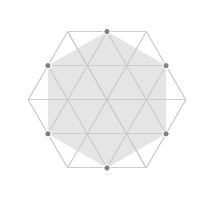
\begin{tikzpicture}[scale=1, transform shape]
    \begin{rootSystem}{A} \roots \end{rootSystem} \end{tikzpicture}
\end{center} \caption{The $A_2$ root system}% \label{fig:} \end{figure}


This is the root system of $SU(3)$. The next root system, in the case where the
angle is $\pi/4$ is the root system $B_2$ and $C_2$, and it looks like

\begin{figure}[H] \begin{center} 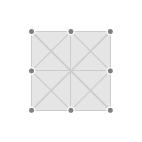
\begin{tikzpicture}[scale=1, transform shape]
    \begin{rootSystem}{B} \roots \end{rootSystem} \end{tikzpicture}
\end{center} \caption{The $B_2$ root system}% \label{fig:} \end{figure}

$B_r$ is the root system of $SO(2r+1)$ and $C_r$ is the root system of
$Sp(2r)$. Next, we have the root system $G_2$, which is drawn below:

\begin{figure}[H] \begin{center} 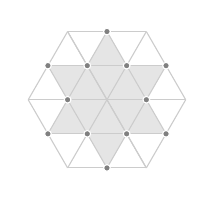
\begin{tikzpicture}[scale=1, transform shape]
    \begin{rootSystem}{G} \roots \end{rootSystem} \end{tikzpicture}
\end{center} \caption{The $G_2$ root system}% \label{fig:} \end{figure}

In general, all finite, or even discrete, groups generated by reflections of
$\R^n$ can be explicitly classified. This restricts to the classification of
crystallographic groups (which preserve a lattice), and inside this we can
classify reduced root systems. This turns out to be the same as classifying
compact Lie groups and complex reductive Lie groups.

The first step is for every $\alpha$, find $r_{\alpha} \in W$. Last time, we
showed that $[\mf{g}_{\alpha}, \mf{g}_{-\alpha}] = \C h_{\alpha} \subset
\mf{t}_{\C}$. Then we know $(h_{\alpha}, h) = c \alpha(h)$. Now we can
normalize this by $\alpha(h_{\alpha}) = 2$. In fact, we will see that the
$h_{\alpha}$ form the dual root system in $\mf{t}$. Next, for any $\alpha$, we
can choose $e_{\alpha} \in \mf{g}_{\alpha}$, which defines an action of
$\mf{sl}(2)$ on $\mf{g}_{\C}$. In particular, we have \[ [e_{\alpha},
\mf{g}_{\beta}] = \mf{g}_{\beta + \alpha} \qquad [e_{-\alpha}, \mf{g}_{\beta}]
= \mf{g}_{\beta - \alpha}. \] Therefore a root $\beta$ corresponds to the
submodule $\bigoplus \mf{g}_{\beta + n \alpha}$, and in particular, we have the
submodule \[ \bigoplus_{n \neq 0} \mf{g}_{n\alpha} \oplus \C h_{\alpha} \] and
so $h_{\alpha}$ is the unique vector of zero weight. Now we know the
representation theory of $SL(2)$, where the highest weights are integers. Also
note that we only have even weights and a unique vector of weight $0$, and thus
the representation above is irreducible. However, by construction, it contains
$\mf{g}_{\alpha} \oplus \mf{g}_{-\alpha} \oplus \C h_{\alpha}$ as a
subrepresentation, so we must have \[ \C h_{\alpha} \oplus \bigoplus_{n \neq 0}
\mf{g}_{n \alpha} = \mf{g}_{\alpha} \oplus \mf{g}_{-\alpha} \oplus \C
h_{\alpha}. \] This proves that $\dim \mf{g}_{\alpha} = 1$ and that the
$\alpha$ are reduced. Also, we know that in the diagram \begin{figure}[H]
    \centering \includegraphics[scale=0.6]{rootstring} \caption{Root String}%
\label{fig:rootstring} \end{figure} the representation $\bigoplus_n
\mf{g}_{\beta + n \alpha}$ is irreducible. These are reversed by $r_{\alpha} =
\mqty(0 & 1 \\ - 1 & 0)$, and thus $\Ad(r_{\alpha})$ acts by reflection on
$\mf{t}$ and $\mf{t}^*$. This implies that \[ 2 \frac{(\alpha, \beta)}{(\alpha,
\alpha)} \in \Z. \]

Our next goal is to show that $W$ is generated by the $r_{\alpha}$. Before we
do this, we will discuss the group generated by reflections. For example, if we
consider an equilateral triangle, we can find a discrete group generated by
reflections.  \begin{figure}[H] \centering
    \includegraphics[scale=0.6]{reflection.png} \caption{Reflection
    hyperplanes}% \label{fig:reflection} \end{figure} We can consider the
    connected components of the complement, and these are called
    \textit{polytopes}. These can be studied in $\R^n, S^n, \mathbb{H}^n$, and
    other spaces. Each of these is a finite intersection of half-spaces and is
    called a \textit{polyhedron}. Then if $r_1, \ldots, r_n$ are the
    reflections in the facets of $\Delta$, they generate a group $\Gamma$. Now
    we can rephrase any word in the generators as a path, so for example, we
    have \begin{figure}[H] \centering
        \includegraphics[width=0.8\linewidth]{reflwords} \caption{Words in the
        generators}% \label{fig:reflwords} \end{figure} Similarly, we can
        obtain $r_1 r_2 r_3 \Delta$ by the procedure \[ \Delta \to r_1 \Delta
        \to r_1 r_2 r_1 (r_1 \Delta) \to r_1 r_2 r_3 r_2 r_1 (r_1 r_2 r_1 (r_1
    \Delta)). \] Therefore, the group $\ev{r_1, r_2, \ldots, r_n}$ acts
    transitively on the set of chambers. In particular, any reflection
    $r_{\alpha}$ is one of these reflections. Now there are some obvious
    relations on the $r_i$: \begin{enumerate} \item Clearly $r_i^2 = 1$.  \item
    If two hyperplanes $r_1, r_2$ have angle $\pi/m$ between them, then we have
    ${(r_1 r_2)}^m = 1$.  \end{enumerate}

\begin{thm} \begin{enumerate} \item This is the complete list of relations
among the $r_i$ \item $\Delta$ is a fundamental domain for $\Gamma$.
\end{enumerate} \end{thm}

The idea of the proof is to remove intersections of hyperplanes of codimension
at least $3$. This is still simply connected, but it has a map \[
\qty{\bigsqcup \Gamma \times \Delta} \to \R^n \setminus \qty{\text{codimension
$\geq 3$ intersections}} \] which is a covering, and therefore it must be an
isomorphism.

To say some more about $W$, if $W$ is generated by relations, recall that $W$
corresponds to critical points on $G/T$ with index $\ell(w)$. Then we will see
that for a vector $\xi$, the relation $\alpha > 0$ if and only if $\alpha(\xi)
> 0$ gives us a chamber for $\ev{r_{\alpha}}$. Therefore by the action of
$\ev{r_{\alpha}}$ we can change the index to be $0$, but there is only one cell
of index $0$ because $G/T$ is connected.

Recall that if $\Gamma$ is a discrete group generated by reflections, a
\textit{chamber} $\Delta$ is a connected component of the complement of the
reflecting hyperplanes.

\begin{thm} \begin{enumerate} \item For a chamber $\Delta$, $\ol{\Delta}$ is a
    fundamental domain for $\Gamma$.  \item $\Gamma$ is in bijection with the
    set of chambers.  \item $\Gamma$ is generated by the reflections $r_i$ in
    the walls of $\Delta$ with the relations $r_i^2 = 1$ and ${(r_i r_j)}^m =
    1$ whenever the walls $r_i, r_j$ have angle $\pi / m$.  \end{enumerate}
\end{thm}

Last time, we proved that the $r_i$ generate $\Gamma$, Next, by the following
picture, we see that words in generators correspond to paths in the set of
chambers: \begin{figure}[H] \centering
    \includegraphics[width=0.8\linewidth]{words} \caption{Words.}%
\label{fig:words} \end{figure}

\begin{proof} We will view words in the generators of a group as the Cayley
    graph. This is the graph with vertices the group elements and edges
    $\gamma_1 \xrightarrow{r_i} \gamma_2$ if $\gamma_2 = r_i \gamma_1$. Because
    $r_i^2 = 1$, we don't need these orientations. Now let \[ \wtl{\Gamma} =
    \ev{r_i} / (r_i^2 = 1, {(r_i, r_j)}^{m_{ij}} = 1) \to \Gamma \to
\qty{\text{chambers}} \] be given by $\gamma \mapsto \gamma \Delta$. This takes
the Cayley graph of $\wtl{\Gamma}$ to the adjacency graph of chambers. We will
prove this map is an isomorphism. This will imply that $\wtl{\Gamma} = \Gamma$
and that $\Gamma$ acts freely on the set of chambers. In fact, we will beef it
up to a covering map of something simply-connected.

    Consider the complement of the codimension $3$ strata in $\R^n$. Also
    consider the set \[ \wtl{\Gamma} \times (\Delta^3 \setminus
    \qty{\text{vertices}}) / ~ \] where we identify $\gamma \times \Delta$ with
    $\gamma r_i \times \Delta$. This is clearly a local isomorphism near points
    on codimension $2$ strata, and therefore is an isomorphism because the
    target is simply connected.  \end{proof}

\begin{exm} Consider the \textit{triangle groups} $\Gamma = \ev{r_1, r_2, r_3}
    / (r_i^2 = 1, {(r_i r_j)}^{m_{ij}} = 1)$. This is the reflection group of
    either $\R^2, S^2, \mathbb{H}^2$ generated by a triangle with angles
    $\frac{\pi}{m_{12}}, \frac{\pi}{m_{13}}, \frac{\pi}{m_{23}}$. Here, the
    cases are \[ \frac{1}{m_{12}} + \frac{1}{m_{23}} + \frac{1}{m_{13}} =
        \begin{cases} > 1 & \Delta \in S^2 \\ 1 & \Delta \in \R^2 \\ < 1 &
        \Delta \in \mathbb{H}^2.  \end{cases} \] For example, consider the
        triangle generated by three perpendicular great circles on the sphere.
        Each angle is $\frac{\pi}{2}$. In $\R^2$, we can consider the tiling of
        the plane by usual equilateral triangles, and in the hyperbolic plane,
        the fundamental domain of the $SL(2, \Z)$ action gives us a
        $(2,3,\infty)$ triangle.  \begin{figure}[H] \centering
            \includegraphics[width=0.8\linewidth]{triangles.png}
            \caption{Triangles}% \label{fig:triangles} \end{figure} In these
            cases, we know $\Gamma$ is \begin{itemize} \item Finite if $\sum
                \frac{1}{m_{ij}} > 1$.  \item Infinite of growth like $R^2$ for
        $\sum \frac{1}{m_{ij}} = 1$.  \item Infinite of exponential growth if
$\sum \frac{1}{m_{ij}} < 1$.  \end{itemize} \end{exm}

Recall that the Weyl group $W = N(T) / T$ is a finite group. 

\begin{thm} $W$ is generated by the $r_{\alpha}$ for all roots $\alpha$.
\end{thm}

\begin{proof} Identify $W$ with the critical points of $(\xi, -)$ on the orbit
    of $\xi$ in $\mf{g}$ for a generic $\xi \in \ms{Lie}(T)$. We need to prove
    that there exists no $w \in W$ such that $w \xi$ is in the same chamber as
    $\xi$. On the critical point $w \xi$, we will compute the index of the
    function $(\xi, -)$. We know this is the number of roots $\alpha$ such that
    $\alpha(\xi) > 0$ and $\alpha(w \xi) < 0$, which is the same as the number
    of hyperplanes separating $\xi$ and $w \xi$. This also equals the number of
    reflecting hyperplanes separating $\Delta$ from $w \Delta$, which is the
    length of $w$.

    Therefore, if there exists $w\xi$ in the same chamber as $\xi$, then there
is more than one maximum of $(\xi, -)$. However, because there are no
$1$-cells, the orbit of $\xi$ is disconnected, which is impossible because $G$
is connected.  \end{proof}

Now we have the following correspondence: \[ \text{Compact group} \to
\text{root system} \to \text{finite reflection group} \subset \text{discrete
reflection groups}. \] Discrete reflection groups in $\R^n$ can be classified,
so from this we can infer a classification of root systems. Next, the map from
compact groups to root systems is an isomorphism, so compact groups (or complex
reductive groups) can be classified. The conclusion is \begin{itemize} \item
    There are four infinite series $SU(n+1), SO(2n+1), Sp(2n), SO(2n)$ denoted
    by $A_n (n \geq 2), B_n (n \geq 2), C_n (n \geq 3), D_n (n \geq 4)$
    corresponding to the different Dynkin diagrams.  \item There are several
    simple exceptional groups: $G_2, E_6, E_7, E_8, F_2$. As a representation
    of $\mf{sl}_3$, we have $\mf{g}_2 = \mf{sl}_3 \oplus \C^3 \oplus
    {(\C^3)}^{\vee}$. Note that $\mf{sl}_3$ has an outer automorphism, which is
    $A \mapsto -A^T$. From this decomposition and the root system, one can
    reconstruct the remaining brackets.  \end{itemize}

Now a \textit{Dynkin diagram} is a diagram with vertices the $r_i$ and an edge
between $r_i$ and $r_j$ when $m_{ij} = 3$ and no edge when $m_{ij} = 2$. When
$m_{ij} = 4$, we have to choose which edge is longer, so the Dynkin diagrams
are \begin{align*} A_n &= \dynkin A{} \\ B_n &= \dynkin B{} \\ C_n &= \dynkin
C{} \\ D_n &= \dynkin D{} \\ E_6 &= \dynkin E6 \\ E_7 &= \dynkin E7 \\ E_8 &=
\dynkin E8 \\ F_4 &= \dynkin F4 \\ G_2 &= \dynkin G2 \end{align*}

\chapter{Bonus: $E_6, E_7, E_8$ and algebraic surfaces}%
\label{cha:bonus_e_6_e_7_e_8_and_algebraic_surfaces}

Recall that algebraic curves (or compact Riemann surfaces) come in three forms:
$\P^1$ (genus $0$, Fano), elliptic curves ($g=1$, Calabi-Yau), and curves of
genus $g > 1$ (general type). Each of these exhibits very different behavior
when we consider meromorphic differentials $\omega$. Then if we consider the
canonical class $K_C \coloneqq (\omega)$. For any two meromorphic differentials
$\omega, \omega'$, we see that $\omega / \omega'$ is a rational function, so
all forms define the same element of $\Pic C$. Also, we can compute using
Riemann-Roch that $\deg K_C = 2g-2$.

For example, on $\P^1$, the form $\dd{x}$ has a double pole at infinity. Then
if we consider a rational function $f \colon C \to \P^1$, we can consider the
form $f^* \dd{x}$ and then compute the degree using Riemann-Hurwitz. This
implies that when $g = 0$, $K_C$ has negative degree, when $g=1$, the degree is
zero, and when $g>0$, the degree is positive.

For general algebraic varieties $X$, we can consider the canonical divisor
$K_X$ associated to a meromorphic top form. Now let $S$ be a smooth projective
surface in $\P^N$. 

\begin{exm} The simplest such $S$ is $\P^2$, and we can consider the form
    $\dd{x} \wedge \dd{y}$ on $\C^2 \subset \P^2$, and this will have a triple
    pole at the line at infinity. Alternatively, if we consider the form
    $\frac{\dd{x}}{x} \wedge \frac{\dd{y}}{y}$, this has poles on the toric
    boundary. This implies that $K_{\P^2} = -3H$, which is the hyperplane
    class.  \end{exm}

\begin{exm} Let $S_d \subset \P^3$ be a surface cut out by a polynomial of
    degree $d$. When $d = 2$, we have a quadric surface, which look like this:
    \begin{figure}[H] \centering \includegraphics[scale=0.8]{quadric}
        \caption{Quadric Surface}% \label{fig:quadric} \end{figure} This has
        two families of lines parameterized by $\P^1$, and in fact, $S_2 \simeq
        \P^1 \times \P^1$. Note that this is \textit{birational} to $\P^2$ but
        is not isomorphic. Projection from a point $x_0 \in S_2$ is a map $S_2
        \dashrightarrow \P^2$ and is an isomorphism outside of the projection
        point and the two lines through it. In fact, to resolve the base point
        of this map, we need to blow up $x_0$. The two rulings through $x_0$
        are contracted. Here, blowup replaces a point by a line representing
        all tangent directions through it.  \begin{figure}[H] \centering
            \includegraphics[scale=1]{blowup.png} \caption{Blowup of a smooth
            point on a surface}% \label{fig:blowup} \end{figure} In the toric
            picture, blowup and blow down are represented by the following:
            \begin{figure}[H] \centering \includegraphics[scale=0.8]{Toric}
                \caption{Toric blowup and blowdown}% \label{fig:Toric}
            \end{figure} Then we obtain $K_{\P^1 \times \P^1} = -2 \mr{pt}
            \times \P^1 - 2 \P^1 \times \mr{pt} = -2H$ because the hyperplane
            section is the sum of two $\P^1$.  \end{exm}

In general, we can compute the canonical class of a hypersurface $\qty{P=0} = Y
\subset X$ using the \textit{adjunction formula}. We can write $\omega_Y =
\frac{\omega_X}{\dd{P}}$ and thus we have \[ K_Y = \eval{(K_X + Y)}_{Y}. \] For
example, if $Y = S_d \subset X = \P^3$, we see that $K_{S_d} = (d-4)H$. This
tells us that \begin{itemize} \item When $d = 1,2,3$, the surface $S_d$ is a
\textit{del Pezzo surface}.  \item When $d=4$, we have a K3 surface.  \item
When $d > 4$, we have a surface of general type.  \end{itemize}

When $d = 3$, the surface is a cubic surface and looks like this:
\begin{figure}[H] \centering \includegraphics[scale=1]{cubicsurf.png}
    \caption{Cubic Surface}% \label{fig:} \end{figure} Over $\C$, every smooth
    cubic surface has $27$ lines. We have $K_S = -H$ and thus $-K_S = H$, which
    is \textit{ample}. Recall that a divisor is ample if some multiple of it
    defines an embedding into $\P^N$. Now there is a map $\Pic S \to
    \mr{NS}(S)$ from the Picard group to the Neron-Severi group, which is the
    group of divisors modulo numerical equivalence. Here, we need the
    intersection form $D_1 \cdot D_2 \in \Z$, which is additive, invariant
    under deformation, and counts intersection points with multiplicity when
    $D_1 \cap D_2$ is discrete and $D_1, D_2$ are \textit{effective}. Here are
    some basic results: \begin{enumerate} \item The Neron-Severi group of a
    surface is a free abelian group $\Z^{\rho}$, and $\rho$ is called the
    \textit{Picard rank}.  \item The signature of the intersection form is $(1,
    \rho -1)$.  \end{enumerate} Inside the cone where $C^2 = 0$, we can
    consider the \textit{ample cone} of ample divisors. The dual of this is the
    closure of the effective cone. There are effective divisors with negative
    self-intersection, for example any line on a cubic surface.

Now we may prove that the cubic surface is rational. To do this, we choose two
skew lines $L, L'$. Now for any points $x, x' \in L, L'$, we consider the line
through $x,x'$ in $\P^3$, and there is a third intersection point. This defines
a birational map $S \dashrightarrow \P^2$, and in fact $S$ is the blowup of
$\P^2$ at six points. When we blow up, we obtain $K_{S} = K_{\P^2} +
\sum_{i=1}^6 E_i$, and thus we have $K^2 = 9-6 = 3$. Thus $-K$ is very ample
and defined an embedding into $\P^3$.This tells us that \[ \Pic S = \Z H \oplus
\bigoplus_{i=1}^6 \Z E_i. \] If $-K_S$ is in the closure of the ample cone and
$C \subset S$ is a curve, we will consider how small $C^2$ can be. By the
adjunction formula, we have \[ g(C) = \frac{C^2 + C \cdot K}{2} +1 \geq 0. \]
Therefore, we have $C^2 \geq -2 -K \cdot C$. Thus we have $-K \cdot C \geq 0$
and this is positive when $-K$ is ample. This implies that $C^2 \geq -2$, and
this happens when $K \cdot C = 0$. If $C^2=-1$, then $C$ is a line and can be
contracted by Castelnuovo's criterion, and when $C^2=-2$, we can contract this
to an $A_1$ singularity (or $\frac{1}{2}(1,1)$). If we consider the
perpendicular of $-K$, then all $(-1)$-curves are: \begin{itemize} \item $C =
E_i$; \item $H - E_i - E_j$; \item $2H - \sum_{k=1}^5 E_{i_k}$.  \end{itemize}
This gives us the $27$ lines on a cubic surface: the six exceptionals, the
strict transforms of the $15$ lines between two of the blown up points, and the
$6$ conics passing through five of the six points. The $(-2)$-curves are:
\begin{itemize} \item $C = E_i - E_j$; \item $C = H - \sum_{i=1}^3 E_i$; \item
$C = 2H - \sum_{i=1}^6 E_i$; \item $C = 3H - 2E_1 - \sum_{i=2}^8 E_i$.
\end{itemize} The first corresponds to blowing up a point twice, the second
corresponds to blowing up three points on a line, and the third corresponds to
blowing up six points on a conic. The last one corresponds to a cubic with a
double point at $p_1$ and seven more points. The last ones correspond to the
roots of $E_6, E_7, E_8$. To see this, if we consider a singular $S_0$ and
nearby nonsingular $S_t$, we have a vanishing cycle in $H^2(S_t)$, which is a
root. If we consider the monodromy, this is exactly the reflection in this
root.

This defines a map from $H^2(S, \Z)$ to the family of all nonsingular cubic
surfaces. Unfortunately, we did not get to the punchline, which was to actually
choose a set of roots in this cohomology.


\end{document}
